% Options for packages loaded elsewhere
% Options for packages loaded elsewhere
\PassOptionsToPackage{unicode}{hyperref}
\PassOptionsToPackage{hyphens}{url}
\PassOptionsToPackage{dvipsnames,svgnames,x11names}{xcolor}
%
\documentclass[
  11pt,
  authoryear,
  doubleblind,
  3p]{elsarticle}
\usepackage{xcolor}
\usepackage{amsmath,amssymb}
\setcounter{secnumdepth}{5}
\usepackage{iftex}
\ifPDFTeX
  \usepackage[T1]{fontenc}
  \usepackage[utf8]{inputenc}
  \usepackage{textcomp} % provide euro and other symbols
\else % if luatex or xetex
  \usepackage{unicode-math} % this also loads fontspec
  \defaultfontfeatures{Scale=MatchLowercase}
  \defaultfontfeatures[\rmfamily]{Ligatures=TeX,Scale=1}
\fi
\usepackage{lmodern}
\ifPDFTeX\else
  % xetex/luatex font selection
\fi
% Use upquote if available, for straight quotes in verbatim environments
\IfFileExists{upquote.sty}{\usepackage{upquote}}{}
\IfFileExists{microtype.sty}{% use microtype if available
  \usepackage[]{microtype}
  \UseMicrotypeSet[protrusion]{basicmath} % disable protrusion for tt fonts
}{}
\makeatletter
\@ifundefined{KOMAClassName}{% if non-KOMA class
  \IfFileExists{parskip.sty}{%
    \usepackage{parskip}
  }{% else
    \setlength{\parindent}{0pt}
    \setlength{\parskip}{6pt plus 2pt minus 1pt}}
}{% if KOMA class
  \KOMAoptions{parskip=half}}
\makeatother
% Make \paragraph and \subparagraph free-standing
\makeatletter
\ifx\paragraph\undefined\else
  \let\oldparagraph\paragraph
  \renewcommand{\paragraph}{
    \@ifstar
      \xxxParagraphStar
      \xxxParagraphNoStar
  }
  \newcommand{\xxxParagraphStar}[1]{\oldparagraph*{#1}\mbox{}}
  \newcommand{\xxxParagraphNoStar}[1]{\oldparagraph{#1}\mbox{}}
\fi
\ifx\subparagraph\undefined\else
  \let\oldsubparagraph\subparagraph
  \renewcommand{\subparagraph}{
    \@ifstar
      \xxxSubParagraphStar
      \xxxSubParagraphNoStar
  }
  \newcommand{\xxxSubParagraphStar}[1]{\oldsubparagraph*{#1}\mbox{}}
  \newcommand{\xxxSubParagraphNoStar}[1]{\oldsubparagraph{#1}\mbox{}}
\fi
\makeatother


\usepackage{longtable,booktabs,array}
\usepackage{calc} % for calculating minipage widths
% Correct order of tables after \paragraph or \subparagraph
\usepackage{etoolbox}
\makeatletter
\patchcmd\longtable{\par}{\if@noskipsec\mbox{}\fi\par}{}{}
\makeatother
% Allow footnotes in longtable head/foot
\IfFileExists{footnotehyper.sty}{\usepackage{footnotehyper}}{\usepackage{footnote}}
\makesavenoteenv{longtable}
\usepackage{graphicx}
\makeatletter
\newsavebox\pandoc@box
\newcommand*\pandocbounded[1]{% scales image to fit in text height/width
  \sbox\pandoc@box{#1}%
  \Gscale@div\@tempa{\textheight}{\dimexpr\ht\pandoc@box+\dp\pandoc@box\relax}%
  \Gscale@div\@tempb{\linewidth}{\wd\pandoc@box}%
  \ifdim\@tempb\p@<\@tempa\p@\let\@tempa\@tempb\fi% select the smaller of both
  \ifdim\@tempa\p@<\p@\scalebox{\@tempa}{\usebox\pandoc@box}%
  \else\usebox{\pandoc@box}%
  \fi%
}
% Set default figure placement to htbp
\def\fps@figure{htbp}
\makeatother





\setlength{\emergencystretch}{3em} % prevent overfull lines

\providecommand{\tightlist}{%
  \setlength{\itemsep}{0pt}\setlength{\parskip}{0pt}}



 
\usepackage[]{natbib}
\bibliographystyle{elsarticle-harv}


\usepackage{xcolor}
\definecolor{revgreen}{HTML}{228B22}

% Block version (paragraphs)
\newenvironment{revision}{\color{revgreen}}{}

% Inline version (phrases/sentences, safe with citations)
\DeclareRobustCommand{\rev}[1]{{\color{revgreen}#1}}
\usepackage{booktabs}
\usepackage{longtable}
\usepackage{array}
\usepackage{multirow}
\usepackage{wrapfig}
\usepackage{float}
\usepackage{colortbl}
\usepackage{pdflscape}
\usepackage{tabu}
\usepackage{threeparttable}
\usepackage{threeparttablex}
\usepackage[normalem]{ulem}
\usepackage{makecell}
\usepackage{xcolor}
\usepackage{setspace}
\onehalfspacing
\geometry{margin=1in}
\usepackage{todonotes,mathtools,bm,amsmath,mathpazo}
\usepackage[linesnumbered,ruled,vlined]{algorithm2e}
\setlength{\parindent}{0cm}
\usepackage{tikz}
\usetikzlibrary{
    arrows.meta,
    positioning,
    fit,
    calc,
    shapes.misc,
    shapes.multipart
  }
\makeatletter
\@ifpackageloaded{caption}{}{\usepackage{caption}}
\AtBeginDocument{%
\ifdefined\contentsname
  \renewcommand*\contentsname{Table of contents}
\else
  \newcommand\contentsname{Table of contents}
\fi
\ifdefined\listfigurename
  \renewcommand*\listfigurename{List of Figures}
\else
  \newcommand\listfigurename{List of Figures}
\fi
\ifdefined\listtablename
  \renewcommand*\listtablename{List of Tables}
\else
  \newcommand\listtablename{List of Tables}
\fi
\ifdefined\figurename
  \renewcommand*\figurename{Figure}
\else
  \newcommand\figurename{Figure}
\fi
\ifdefined\tablename
  \renewcommand*\tablename{Table}
\else
  \newcommand\tablename{Table}
\fi
}
\@ifpackageloaded{float}{}{\usepackage{float}}
\floatstyle{ruled}
\@ifundefined{c@chapter}{\newfloat{codelisting}{h}{lop}}{\newfloat{codelisting}{h}{lop}[chapter]}
\floatname{codelisting}{Listing}
\newcommand*\listoflistings{\listof{codelisting}{List of Listings}}
\makeatother
\makeatletter
\makeatother
\makeatletter
\@ifpackageloaded{caption}{}{\usepackage{caption}}
\@ifpackageloaded{subcaption}{}{\usepackage{subcaption}}
\makeatother
\journal{Production and Operations Management}
\usepackage{bookmark}
\IfFileExists{xurl.sty}{\usepackage{xurl}}{} % add URL line breaks if available
\urlstyle{same}
\hypersetup{
  pdftitle={Estimating censored demand in family planning supply chains: forecast accuracy, inventory implications, and public health outcomes},
  pdfauthor={Harsha Chamara Hewage; Bahman Rostami-Tabar; Aris Syntetos; Federico Liberatore; Glenn R. Milano},
  pdfkeywords={Censored Demand Forecasting, Tobit Kalman
Filter, Conformal Prediction, Inventory Planning, Family Planning Supply
Chains},
  colorlinks=true,
  linkcolor={blue},
  filecolor={Maroon},
  citecolor={Blue},
  urlcolor={Blue},
  pdfcreator={LaTeX via pandoc}}


\setlength{\parindent}{6pt}
\begin{document}
% Added cover page only; all spacing/font changes are local to this group.
\begingroup
\thispagestyle{plain}
\singlespacing
\setlength{\parindent}{0pt}
\setlength{\parskip}{0pt}
{\centering\Large\bfseries Estimating censored demand in family planning supply chains: forecast accuracy, inventory implications, and public health outcomes\par}
\vspace{1.5em}

\noindent\begin{minipage}{\linewidth}
\textbf{Harsha Chamara Hewage} (Corresponding author)\par
Data Lab for Social Good Research Group, Cardiff Business School\par
Cardiff University\par
Aberconway Building, Colum Drive\par
Cardiff, CF10 3EU, United Kingdom\par
\href{mailto:HalgamuweHewageHR@cardiff.ac.uk}{HalgamuweHewageHR@cardiff.ac.uk}\par
\end{minipage}\par\vspace{1em}

\noindent\begin{minipage}{\linewidth}
\textbf{Bahman Rostami-Tabar}\par
Data Lab for Social Good Research Group, Cardiff Business School\par
Cardiff University\par
Aberconway Building, Colum Drive\par
Cardiff, CF10 3EU, United Kingdom\par
\href{mailto:rostami-tabarb@cardiff.ac.uk}{rostami-tabarb@cardiff.ac.uk}\par
\end{minipage}\par\vspace{1em}

\noindent\begin{minipage}{\linewidth}
\textbf{Aris Syntetos}\par
PARC Institute of Manufacturing, Logistics \& Inventory\par
Cardiff Business School\par
Cardiff University\par
Aberconway Building, Colum Drive\par
Cardiff, CF10 3EU, United Kingdom\par
\href{mailto:syntetosa@cardiff.ac.uk}{syntetosa@cardiff.ac.uk}\par
\end{minipage}\par\vspace{1em}

\noindent\begin{minipage}{\linewidth}
\textbf{Federico Liberatore}\par
Cardiff School of Computer Science \& Informatics\par
Cardiff University\par
Abacws building, Senghennydd Road, Cathays\par
Cardiff, CF24 4AG, United Kingdom\par
\href{mailto:liberatoref@cardiff.ac.uk}{liberatoref@cardiff.ac.uk}\par
\end{minipage}\par\vspace{1em}

\noindent\begin{minipage}{\linewidth}
\textbf{Glenn R. Milano}\par
Bureau for Global Health\par
United States Agency for International Development (Former)\par
20523, United States\par
\href{mailto:glenn.milano@gmail.com}{glenn.milano@gmail.com}\par
\end{minipage}\par
\endgroup
\clearpage

% Keep the Elsevier abstract/keyword boxes, but omit the repeated title
% and the two horizontal rules on the manuscript's opening page.
\let\pomOriginalMaketitleBox\MaketitleBox
\renewcommand{\MaketitleBox}{%
  \resetTitleCounters
  \begingroup
    \def\baselinestretch{1}%
    \setlength{\parskip}{0pt}%
    \ifvoid\absbox\else\unvbox\absbox\par\vskip10pt\fi
    \ifvoid\keybox\else\unvbox\keybox\par\fi
  \endgroup
}

\begin{frontmatter}
\title{Estimating censored demand in family planning supply chains:
forecast accuracy, inventory implications, and public health outcomes}
\author[1]{Harsha Chamara Hewage%
\corref{cor1}%
}
 \ead{HalgamuweHewageHR@cardiff.ac.uk} 
\author[1]{Bahman Rostami-Tabar%
%
}
 \ead{rostami-tabarb@cardiff.ac.uk} 
\author[2]{Aris Syntetos%
%
}
 \ead{syntetosa@cardiff.ac.uk} 
\author[3]{Federico Liberatore%
%
}
 \ead{liberatoref@cardiff.ac.uk} 
\author[4]{Glenn R. Milano%
%
}
 \ead{glenn.milano@gmail.com} 

\affiliation[1]{organization={Cardiff University, Data Lab for Social
Good Research Group, Cardiff Business School},country={United
Kingdom},countrysep={,},postcode={CF10 3EU},postcodesep={}}
\affiliation[2]{organization={Cardiff University, PARC Institute of
Manufacturing, Logistics \& Inventory, Cardiff Business
School},country={United Kingdom},countrysep={,},postcode={CF10
3EU},postcodesep={}}
\affiliation[3]{organization={Cardiff University, Cardiff School of
Computer Science \& Informatics},country={United
Kingdom},countrysep={,},postcode={CF24 4AG},postcodesep={}}
\affiliation[4]{organization={United States Agency for International
Development (Former), Bureau for Global Health},country={United
States},countrysep={,},postcode={20523},postcodesep={}}

\cortext[cor1]{Corresponding author}





        
\begin{abstract}
\begin{singlespace}
Lost sales due to stockouts and service interruptions create a major challenge for demand forecasting in family planning supply chains. When demand is censored, forecasts become biased, reinforcing cycles of understocking and unmet need. Existing models often ignore this distortion or treat all censoring mechanisms uniformly, limiting their decision relevance in operational settings. We propose the Truncated Conformal Kalman Filter (TCKF), a novel forecasting framework that integrates a Tobit Kalman Filter with conformal prediction. Unlike existing approaches, TCKF explicitly distinguishes between partial censoring (stockouts) and full censoring (interruptions or no-stock-received periods), enabling context-sensitive state updates. It also adapts to prolonged uncertainty through dynamic process-noise inflation and generates distribution-free prediction intervals, avoiding restrictive assumptions about error distributions. We evaluate performance using both synthetic and real-world data from the family planning program in Côte d’Ivoire, and we assess the impact on public health outcomes. Across both settings, TCKF consistently outperforms benchmark methods in forecast accuracy, considering both point and probabilistic forecasts, as well as in downstream inventory performance. Moreover, our results show how improvements in forecast accuracy can translate into better product availability and enhanced public health outcomes. This work bridges a critical gap between forecasting and inventory control and offers a scalable solution for supply chains facing censored demand.
\end{singlespace}
\end{abstract}





\begin{keyword}
    Censored Demand Forecasting \sep Tobit Kalman Filter \sep Conformal
Prediction \sep Inventory Planning \sep 
    Family Planning Supply Chains
\par\smallskip
\noindent Received: November 2025; revised: January, May, August and
September 2026; accepted: November 2026 by Christopher Tang after four
revisions.
\end{keyword}
\end{frontmatter}
\thispagestyle{plain}
\let\MaketitleBox\pomOriginalMaketitleBox
    

\section{Introduction}\label{sec-intro_wp2}

Reliable demand forecasting is foundational to the functioning of Family
Planning Supply Chains (FPSC), directly shaping contraceptive
availability, service delivery, and health outcomes \citep{hewage2025}.
Even small improvements in availability can lead to measurable increases
in uptake. For instance, having one additional method available can
result in a 6.5\% increase in contraceptive usage
\citep{rosen2018modeling}. Yet, generating accurate forecasts in FPSC
settings remains a persistent challenge due to volatile demand patterns,
poor data quality, and operational disruptions such as frequent
stockouts and service interruptions \citep{karimi2021, devries2020}. In
fact, fewer than half of health facilities in some settings maintain
records in LMIS (Logistics Management Information System) that match
their physical inventory counts \citep{karimi2021}.

These structural and operational constraints frequently lead to censored
demand data, periods where actual need is unobserved or underreported.
In FPSC, two main forms of censoring arise (see
Figure~\ref{fig-ts_plot_wp2}). First, \textbf{partial censoring} occurs
during stockouts, where true demand exceeds available inventory and
healthcare sites can only record sales up to the amount of stock on hand
\citep{karimi2021}. Second, \textbf{full censoring} arises from service
interruptions, including facility closures, undertrained staff, or data
collection failures, which prevent actual demand from being recorded at
all \citep{hewage2025, muyinda2015}. For example, a health facility
might report zero demand because it was closed, even when products were
available in the system and users needed them.

\begin{figure}

\centering{

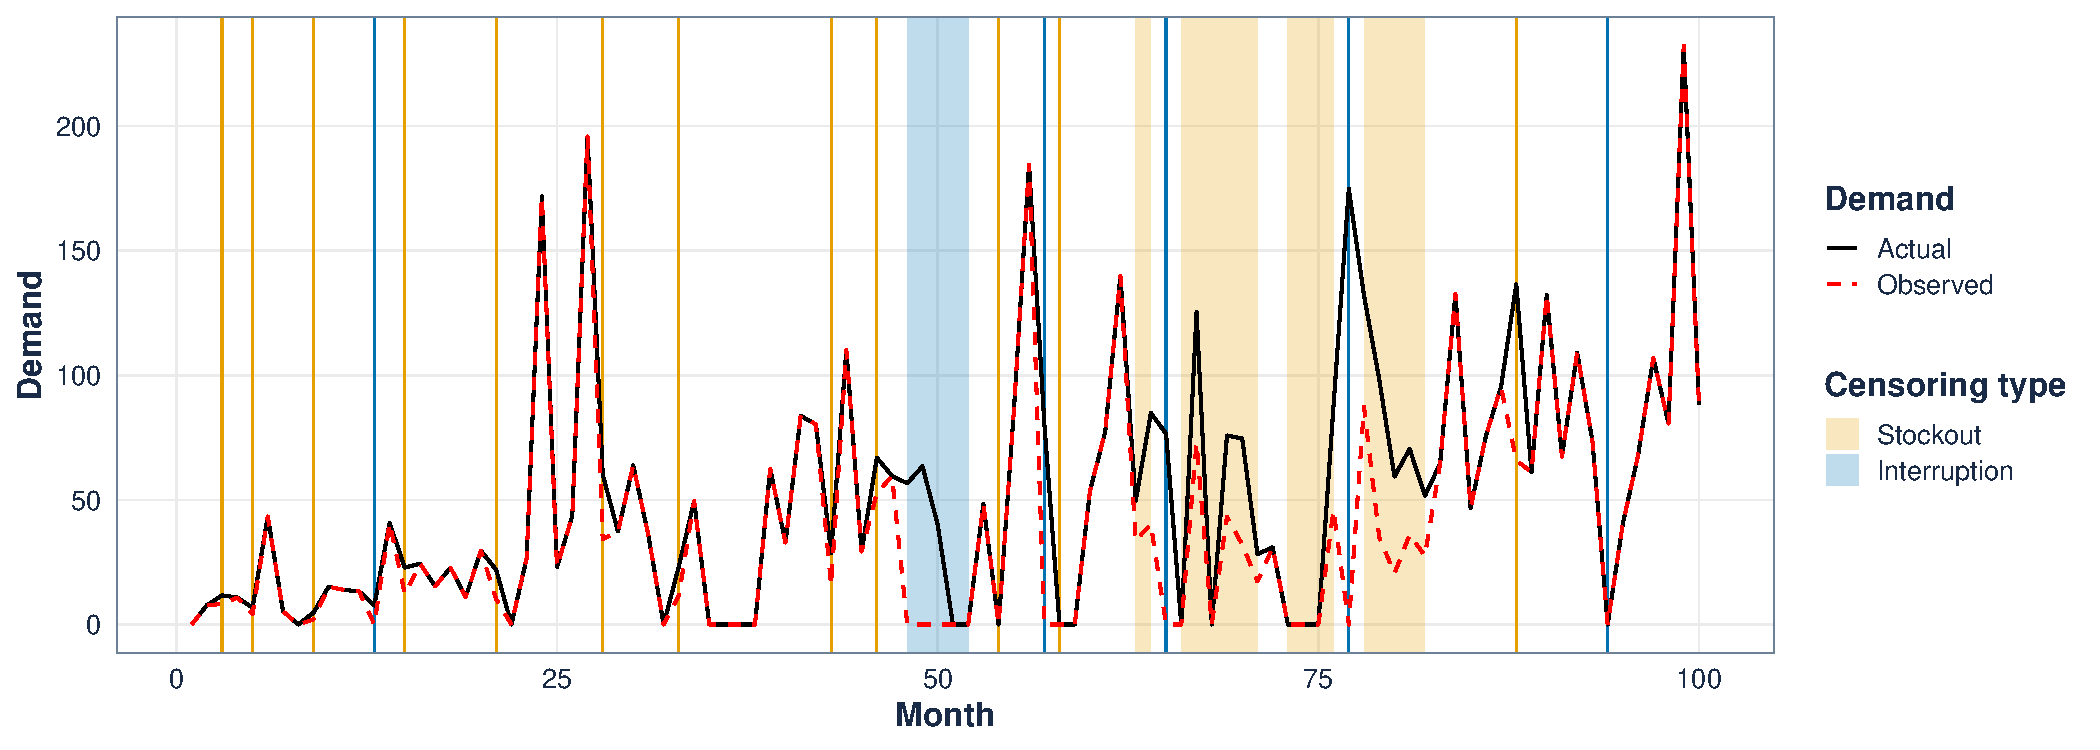
\includegraphics[width=0.7\linewidth,height=\textheight,keepaspectratio]{Main-Paper-Figure-01.pdf}

}

\caption{\label{fig-ts_plot_wp2}Censoring scenarios in family planning
supply chains.}

\end{figure}%

The failure to capture true demand results in systematically biased
sales records and downward-biased forecasts
\citep{wecker1978, trapero2024}. This situation is referred to as a
\textbf{lost sales context} in inventory management \citep{heese2010},
where the true extent of unmet demand remains unknown. Ignoring
censoring leads to under-ordering, increased risk of stockouts, and a
\textbf{spiral-down effect}, where misinformed replenishment decisions
lead to further unmet need and lost sales over time \citep{cooper2006}.

While the lost sales framework is widely used in inventory theory to
distinguish between systems with and without backordering, it rarely
considers how those losses arise from structural data issues. In FPSC,
lost sales refer to unmet consumption or distribution opportunities,
demand that goes unrecorded due to stockouts or service interruptions,
rather than commercial transactions. In such systems, demand cannot be
backordered; if a user visits during a stockout, that opportunity is
permanently lost. For example, methods like emergency contraceptives are
time-sensitive, and their need does not carry over. Here, censoring
becomes the mechanism through which demand is lost. Ignoring this
distinction risks underestimating both need and service risk in
replenishment models.

When contraceptives are unavailable, users may be turned away or forced
to forgo their preferred method \citep{sedgh2016}. Even when
alternatives exist, concerns about switching and the cost of seeking
supplies elsewhere can limit access \citep{karimi2021, RHSC2016}. This
can increase unmet need for family planning and the risk of unintended
pregnancies \citep{sully2020}.

Our discussions with supply chain planners at USAID and with JSI country
teams highlighted similar concerns about stockouts, service
interruptions and incomplete demand information. These engagements
connect the research problem with operational practice. The empirical
analysis uses data from Côte d'Ivoire only.

The existing solutions to tackle the lost sales context remain ad hoc,
depending on available information and specific demand assumptions (see
Table~\ref{tbl-literature_wp2}) \citep{trapero2024}. A core challenge is
the unobserved nature of lost sales, causing biases in data and
complicating forecasting and inventory optimisation
\citep{beutel2012, pedregal}. Many existing methods assume constant
censoring levels or do not distinguish stockouts from service
interruptions. Simple time series models struggle with missing data and
with capturing complex temporal patterns like trends, seasonality, or
external shocks \citep{hewage2025}.

In practice, demand planners often intervene, adjusting System-Generated
forecasts or revising order quantities to account for local realities
not captured in the data \citep{siemsen2025, hewage2025}. These
adjustments may reflect anticipated deliveries, outreach campaigns, or
known reporting gaps, and are often made to prevent stockouts. However,
such interventions are informal, vary across sites, and are rarely
supported by formal tools. Yet, prior studies show that under lost
sales, such adjustments often anchor on available data and under-correct
for unobserved need \citep{feiler2013, tong2018}. While behavioural
tools have been proposed to mitigate this bias, their use in operational
settings remains limited \citep{syntetos2016}. This highlights the need
for forecasting approaches that are structurally aligned with how demand
is recorded and censored in FPSC, reducing reliance on manual
workarounds.

At the same time, optimal inventory policies under lost sales are
computationally intensive due to the curse of dimensionality, where
decisions depend on the full inventory pipeline \citep{bijvank2011}.
Traditional models often assume that excess demand is backordered, an
assumption that does not hold in FPSC, where demand is typically lost if
unfulfilled \citep{karimi2021, hewage2025}. Moreover, the historical
separation of forecasting and inventory research limits understanding of
how demand estimation translates into actual service levels
\citep{goltsos2022}.

To address these limitations, we propose the Truncated Conformal Kalman
Filter (TCKF), a probabilistic forecasting framework specifically
designed to model censored demand and support inventory decision-making
in FPSC. The method integrates a Tobit Kalman Filter with a conformal
prediction layer. The Kalman filter component allows for time series
modelling in the presence of partial and full censoring, while
accounting for trends, shocks, and missing observations. The conformal
layer provides calibrated, distribution-free prediction intervals,
enabling more robust, uncertainty-aware inventory planning. While
individual studies have addressed aspects of forecasting, inventory, or
service access, no prior work in FPSC has offered an integrated approach
that links demand forecast with inventory implications and downstream
public health impact. To our knowledge, this is the first such framework
applied to FPSC. The key contributions of our study are:

\begin{itemize}
\item
  We introduce TCKF, which separates stockouts from service
  interruptions and uses conformal calibration.
\item
  We evaluate the forecasting and inventory performance of TCKF using
  synthetic and empirical data from Côte d'Ivoire, showing how its
  operational value depends on the replenishment policy.
\item
  We translate differences in stockout exposure into potential
  contraceptive access consequences using relative modern contraceptive
  prevalence rate (mCPR)\footnote{The percentage of women of
    reproductive age using modern contraceptive methods} loss,
  connecting inventory performance to its public health relevance.
\end{itemize}

\section{Research background}\label{sec-lit_wp2}

\subsection{The lost sales problem in
FPSC}\label{the-lost-sales-problem-in-fpsc}

Lost sales are a defining challenge in family planning supply chains,
where unmet demand due to stockouts or service interruptions often goes
unrecorded \citep{bijvank2011, trapero2024}. Most empirical work focuses
on the frequency and operational causes of stockouts
\citep{morgan2014, karimi2021}, while planning tools often continue to
treat recorded consumption as complete
\citep{family_planning_logistics_management_fplm_contraceptive_2000, hewage2025}.
This leaves open the question of how censored demand affects forecasting
and replenishment decisions.

\subsection{Forecasting decisions under lost
sales}\label{forecasting-decisions-under-lost-sales}

The issue of censored demand was formally recognised in the forecasting
literature with the Tobit model introduced by \citet{tobin1958}.
Subsequent approaches used exponential smoothing, auxiliary information
or adjustments to observed sales to approximate lost demand
\citep{nahmias1994, lau1996, hyndman_forecasting_2008}. Their
application in FPSC depends on the availability of auxiliary information
or reliable observations from fully stocked periods.

More recently, general-purpose models have been proposed to address the
lost sales forecasting problem more rigorously \citep{wangxu2025}. The
Tobit Kalman Filter (TKF), introduced by \citet{trapero2024}, integrates
state-space modelling with censoring logic, treating observed sales as
censored manifestations of latent demand. TKF captures dynamics such as
trend, seasonality, and external shocks while allowing for time-varying
censoring levels, something earlier models failed to accommodate.
Simulation studies have shown that TKF reduces lost sales and improves
service levels compared to previous heuristic methods.

In parallel, the Tobit Exponential Smoothing (TETS) model extends
exponential smoothing to censored time series using innovations state
space modelling \citep{pedregal, pedregal2026}. TETS is capable of
handling different data frequencies and temporal hierarchies, making it
suitable for retail and health systems where inventory reviews and sales
occur on different time scales. Despite their robustness, models like
TKF and TETS have not yet been applied in FPSC contexts. Although TKF
and TETS address data censoring, they do not explicitly account for the
severe quality issues, discontinuities, and erratic behaviors in
real-world FPSC data.

\subsection{Inventory decisions under lost
sales}\label{inventory-decisions-under-lost-sales}

Inventory control under lost sales remains analytically challenging,
especially with positive lead times and unobserved demand
\citep{bijvank2011, heese2010}. Distribution-free and learning-based
methods have been used to infer lost demand or guide replenishment under
uncertainty \citep{sachs2014, godfrey2001, zheng2026}. More recent work
links probabilistic forecasts to inventory decisions and shows how
decision-aware methods can support the allocation of essential medicines
under limited and noisy data \citep{chung2026}.

\subsection{Literature review gap
summary}\label{literature-review-gap-summary}

Existing research has advanced censored-demand forecasting and inventory
control, but their integration remains limited, particularly in FPSC.
Forecasts are often evaluated on statistical accuracy without assessing
their implications for availability and unmet demand, while inventory
models may assume demand is fully observed \citep{babai2025}. Some
studies have explicitly considered both dimensions, highlighting the
importance of evaluating forecasting methods not only in terms of
statistical accuracy but also their inventory implications
\citep[e.g.,][]{babai2020}. This study examines how distinguishing
stockouts from service interruptions and calibrating forecast
uncertainty can support replenishment decisions. We evaluate forecast
and inventory performance and translate stockout exposure into potential
contraceptive-access consequences. Table~\ref{tbl-literature_wp2}
summarises how the framework relates to existing approaches,
distinguishing its forecasting features from its downstream evaluation.

\begingroup\fontsize{6}{8}\selectfont

\begin{longtable}[t]{>{\raggedright\arraybackslash}p{8em}>{\raggedright\arraybackslash}p{12em}>{\raggedright\arraybackslash}p{12em}>{\raggedright\arraybackslash}p{12em}>{\raggedright\arraybackslash}p{12em}>{\raggedright\arraybackslash}p{8em}}

\caption{\label{tbl-literature_wp2}Overview of the literature summary.}

\tabularnewline

\toprule
Reference & Model/ Method & Censoring type (stockouts/ interruptions) & Probabilistic forecast & Inventory link & Public health impact\\
\midrule
\endfirsthead
\multicolumn{6}{@{}l}{\textit{(continued)}}\\
\toprule
Reference & Model/ Method & Censoring type (stockouts/ interruptions) & Probabilistic forecast & Inventory link & Public health impact\\
\midrule
\endhead

\endfoot
\bottomrule
\endlastfoot
Wecker (1978) & AR Model with Normal Errors & Stockouts & Yes & No & No\\
Nahmias and Smith (1994) & Exp. Smoothing Estimator & Stockouts & Yes & Yes & No\\
Lau \& Lau (1996) & High-Freq Data with Expert Opinion & Stockouts & Yes & No & No\\
Hyndman (2008) & Nonnegative Correction & Stockouts & Yes & No & No\\
Trapero et al. (2024) & TKF & Stockouts & Yes & Yes & No\\
\addlinespace
Pedregal \& Trapero (2024) & TETS with Aggregation & Stockouts & Yes & Yes & No\\
Tong et al. (2018) & REDO & Stockouts & No & No & No\\
Godfrey \& Powell (2001) & CAVE & Stockouts & No & Yes & No\\
Beutel \& Minner (2012) & Data-Driven Newsvendor & Stockouts & No & Yes & No\\
Sachs \& Minner (2014) & Distribution-Free Newsvendor & Stockouts & No & Yes & No\\
\addlinespace
Heese \& Swaminathan (2010) & Bayesian & Stockouts & Yes & Yes & No\\
This study & Truncated Conformal Kalman Filter & Stockouts, Interruptions & Yes & Yes & Yes\\*

\end{longtable}

\endgroup{}

\section{Proposed model: Truncated Conformal Kalman Filter
(TCKF)}\label{sec-model_wp2}

\subsection{Tobit Kalman Filter}\label{tobit-kalman-filter}

To address the challenge of forecasting under censored demand, we first
establish a baseline using the Tobit Kalman Filter (TKF), as proposed by
\citet{trapero2024}. The TKF integrates state-space modelling with
censoring logic, treating observed sales as censored manifestations of a
latent demand process.

Let \(y_t^{*}\) denote the latent (true) demand at time \(t\), which is
assumed to follow a standard state-space structure. For a Local Level
Model (LLM), the state transition and measurement equations are defined
as:

\begin{equation}\phantomsection\label{eq-tkf-main}{
\begin{aligned}
y_t^{*} &= \mu_t + \epsilon_t, \qquad \epsilon_t \sim \mathcal{N}(0, \sigma_{\epsilon}^{2}) \\
\mu_{t+1} &= \mu_t + \eta_t, \qquad \eta_t \sim \mathcal{N}(0, \sigma_{\eta}^{2})
\end{aligned}
}\end{equation}

where \(\mu_t\) represents the level component, and \(\epsilon_t\) and
\(\eta_t\) are independent Gaussian noise terms. In the presence of
inventory constraints, the observed sales \(y_t\) are related to the
latent demand \(y_t^{*}\) via the censoring mechanism:

\begin{equation}\phantomsection\label{eq-tkf-2}{
y_t =
\begin{cases}
y_t^{*}, & \text{if } y_t^{*} \le I_t \\
I_t, & \text{if } y_t^{*} > I_t
\end{cases}
}\end{equation}

where \(I_t\) is the available inventory at time \(t\). The standard TKF
accounts for partial censoring (stockouts) by using a Tobit likelihood
function to update the state estimates when \(y_t = I_t\). In this
framework, the measurement equation is modified to account for the
probability that the true demand lies above the threshold \(I_t\).

However, a key limitation of the standard TKF in public health supply
chains is its inability to distinguish between stockouts (where demand
exceeds supply, providing a lower bound) and service interruptions
(where demand is completely unobservable due to facility closures or
absent staff). Treating interruptions as zero demand biases the forecast
downward, while treating them merely as missing data fails to account
for the increasing uncertainty during the interruptions.

To address these limitations, we propose the TCKF. While TCKF builds on
the Tobit-based framework of \citet{trapero2024} and \citet{pedregal},
it introduces distinct mechanisms for handling the specific disruptions
found in FPSC. Unlike existing approaches, TCKF explicitly distinguishes
between partial censoring and full censoring, enabling context-sensitive
state updates.

\subsection{Problem setup}\label{problem-setup}

Let \(y_t\) denote the observed demand at time \(t\), subject to
potential censoring. We define the true (i.e., latent) demand
\(D_t \in \mathbb{R}{\geq 0}\) as a function of unobserved components
evolving over time:

\begin{equation}\phantomsection\label{eq-one}{
D_t = \ell_t + \tau_t + \gamma_t + \varepsilon_t, \quad \varepsilon_t \sim \mathcal{N}(0, \sigma^2)
}\end{equation}

where \(\ell_t\) is the level, \(\tau_t\) is the trend, \(\gamma_t\) is
the seasonal component, and \(\varepsilon_t\) is Gaussian noise. The
latent state vector is defined as:

\begin{equation}\phantomsection\label{eq-two}{
X_t = \begin{bmatrix} \ell_t \\ \tau_t \\ \gamma_t \end{bmatrix}
}\end{equation}

We assume \(X_t\) evolves according to a state-space model:

\begin{equation}\phantomsection\label{eq-three}{
X_t = F X_{t-1} + \eta_t, \quad \eta_t \sim \mathcal{N}(0, Q_t)
}\end{equation}

where the transition matrix \(F\) and time-varying process noise \(Q_t\)
are:

\begin{equation}\phantomsection\label{eq-four}{
F = \begin{bmatrix} 1 & 1 & 0 \\ 0 & 1 & 0 \\ 0 & 0 & \phi \end{bmatrix}, \quad Q_t = Q_0 + \lambda k_t I, \quad 0 \leq \lambda \leq 1
}\end{equation}

Here, \(\phi \quad in \quad [0,1]\) is the seasonal decay
factor\footnote{If \(\phi = 1\), seasonality remains constant. If
  \(\phi < 1\), the seasonal effect gradually fades.}, \(\lambda\) is a
bias inflation scalar, and \(k_t\) is the number of consecutive censored
observations at time \(t\). The matrix \(Q_t\) increases as censoring
persists to reflect rising model uncertainty.

The observed demand \(y_t\) depends on the availability of stock:

\begin{equation}\phantomsection\label{eq-five}{
y_t = \begin{cases}
H X_t + \nu_t, & \text{if } y_t \text{ is uncensored} \\
0, & \text{if } y_t \text{ is fully censored} \\
\min(H X_t, s_t), & \text{if } y_t \text{ is partially censored}
\end{cases}, \quad \nu_t \sim \mathcal{N}(0, R)
}\end{equation}

where \(s_t\) is available stock at time \(t\),
\(H = [1 \quad 0 \quad 1]\) is the observation matrix (mapping level and
seasonality to the observed signal), and \(R\) is the observation noise
variance.

In the observation matrix \(H\), we define the trend as an internal
\emph{drift} in the system that is folded into the level over time.
Thus, short-term trend variations are not directly measurable in the
observed demand. The trend is inferred over time through the system's
dynamic evolution. In the case of full censoring, instead of treating
the observed value as a literal zero, we model these instances as
right-censored at zero. The likelihood of the observation is then
represented by a truncated Gaussian distribution bounded below by zero,
acknowledging that while the true demand is unobserved, it is known to
be non-negative.

\subsection{Inference with Truncated Kalman
Filter}\label{inference-with-truncated-kalman-filter}

To accommodate censored observations within the Kalman filtering
framework, we incorporate a correction based on the expectation of a
truncated Gaussian distribution. In contrast to standard Kalman
filtering, which assumes Gaussian-distributed observations, here the
observed variable \(y_t\) may be censored due to supply constraints.
This necessitates modifying the update step when \(y_t\) is partially or
fully censored.

The first step in each iteration involves computing the predicted
observation mean and variance:

\begin{equation}\phantomsection\label{eq-six}{
\mu_t = H \hat{X}_{t|t-1}, \quad \sigma^2_t = H P_{t|t-1} H^\top + R
}\end{equation}

Here, \(\mu_t\) is the forecasted mean of the observation, and
\(\sigma^2_t\) is the associated variance, accounting for both state
uncertainty and observation noise.

\subsubsection{Separating stockouts and service
interruptions}\label{sec-model_seperate}

A key extension of TCKF is that it separates two operationally different
forms of censored demand: stockouts and service interruptions. This
distinction matters because the two regimes provide different
information about latent demand.

During a stockout, observed demand is constrained by available stock. If
the stock threshold is \(s_t\), then true demand satisfies
\(D_t \geq s_t\). Under the one-step-ahead forecast distribution
\(D_t \mid \mathcal{F}_{t-1} \sim N(\mu_t,\sigma_t^2)\), the expected
latent demand is

\begin{equation}\phantomsection\label{eq-stockout-conditional-mean}{
\mathbb{E}(D_t \mid D_t \geq s_t)
=
\mu_t+
\sigma_t
\frac{\phi(a_t)}
{1-\Phi(a_t)},
\qquad
a_t=\frac{s_t-\mu_t}{\sigma_t}
}\end{equation}

This conditional expectation is greater than \(\mu_t\), so a stockout
provides useful lower-bound information for updating the demand state. A
service interruption is different. The recorded zero arises because
service was unavailable and therefore does not provide a meaningful
demand threshold. TCKF consequently skips the measurement update and
propagates the prior state, while allowing uncertainty to increase.

This section explains three aspects of regime separation: the conditions
under which a recorded zero carries no additional demand information,
how updating the state using such a zero can introduce estimation error,
and how alternative treatments of that zero affect the innovation and
estimated uncertainty.

We first explain the conditions under which a recorded zero during a
service interruption provides no information for updating the demand
state. Let \(C_t=1\) denote a known service interruption, during which
\(y_t=0\) because service is unavailable. Once the interruption is
known, the recorded zero adds no further information, so

\begin{equation}\phantomsection\label{eq-interruption-state}{
p(X_t \mid y_t=0,C_t=1,\mathcal{F}_{t-1})
=
p(X_t \mid C_t=1,\mathcal{F}_{t-1}).
}\end{equation}

For this distribution to equal the prior
\(p(X_t \mid \mathcal{F}_{t-1})\), the interruption itself must also be
unrelated to the latent demand state, conditional on past information:
\(C_t \perp X_t \mid \mathcal{F}_{t-1}\). This condition applies when
the interruption is caused by operational factors that provide no
additional information about latent demand. Under this condition, and
when the predictive state mean represents the conditional expectation,
\(\hat{X}_{t|t-1}\) remains the minimum mean squared error (MSE)
estimate. This explains why TCKF skips the measurement update during a
known service interruption. If the occurrence of an interruption is
informative about demand, this reasoning does not apply without
modelling that relationship.

We next explain how updating the state using an interruption zero can
introduce estimation error. Consider a comparator that starts from the
same predictive state estimate as TCKF but applies a measurement update
with innovation \(\delta_t\):

\begin{equation}\phantomsection\label{eq-regime}{
\hat{X}^{C}_{t|t}
=
\hat{X}_{t|t-1}
+
K_t\delta_t.
}\end{equation}

Under the conditions above, the prediction error
\(e_t=X_t-\hat{X}_{t|t-1}\) has conditional mean zero. If
\(K_t\delta_t\) is determined by past information and the known
interruption, the cross term in the squared error has conditional
expectation zero. The difference in conditional state-estimation MSE is
therefore

\begin{equation}\phantomsection\label{eq-mse}{
\operatorname{MSE}_{C}
-
\operatorname{MSE}_{TCKF}
=
\lVert K_t\delta_t\rVert^2
\geq 0.
}\end{equation}

The difference is positive when the update changes the state estimate.
This explains the immediate effect of using an uninformative zero in the
measurement update. The comparison concerns a single update from a
common prior under the stated conditions; it does not establish the size
of forecasting or inventory gains over a sequence of periods.

Finally, we explain how two alternative treatments of an interruption
zero affect the innovation. Treating the zero as an ordinary demand
observation gives \(\delta_t^{N}=-\mu_t\). For a positive predicted
mean, this creates a negative innovation and, with a positive level
gain, pulls the estimated demand level downward. Treating the zero as a
censored observation with threshold \(s_t=0\), as in the pooled
specification used in Section~\ref{sec-model_diag}, instead gives, from
Equation~\ref{eq-stockout-conditional-mean},

\begin{equation}\phantomsection\label{eq-pooled-innovation}{
\delta_t^{P}
=
\sigma_t\lambda(r_t)
>
0,
\qquad
\lambda(r)=\frac{\phi(r)}{\Phi(r)},
\qquad
r_t=\frac{\mu_t}{\sigma_t}.
}\end{equation}

This treatment creates a positive innovation and, with a positive level
gain, pushes the estimated demand level upward. For \(r_t\geq0\),
\(\lambda(r_t)\leq\sqrt{2/\pi}\approx0.798\), so the pooled innovation
is at most \(0.798\sigma_t\). The corresponding change in the state is
\(K_t\delta_t^{P}\) and therefore also depends on the gain. Repeated
interruption updates can carry these changes into subsequent forecasts,
although their accumulated effect depends on the state dynamics and
gains.

The pooled treatment also applies a censored-observation variance update
during a period that, under the conditions above, provides no new demand
information. It can therefore reduce the estimated uncertainty without
an informative observation. An upward shift in the forecast mean and a
reduction in forecast dispersion have opposing effects on upper forecast
quantiles, so their net effect on coverage is not determined by this
argument alone. Section~\ref{sec-model_diag} examines the direction and
magnitude of these differences numerically.

\subsubsection{Uncensored Update}\label{uncensored-update}

If the observation \(y_t\) is not subject to censoring, the standard
Kalman update equations apply:

\begin{equation}\phantomsection\label{eq-seven}{
K_t = \frac{P_{t|t-1} H^\top}{\sigma^2_t}, \quad \hat{X}_{t|t} = \hat{X}_{t|t-1} + K_t (y_t - \mu_t)
}\end{equation}

This step updates the state estimate by incorporating the innovation, or
residual, between the actual and predicted observations. The relevant
components are:

\begin{itemize}
\tightlist
\item
  Innovation (residual): \(\tilde{y}_t = y_t - H \hat{X}_{t|t-1}\)
\item
  Innovation covariance: \(S_t = H P_{t|t-1} H^\top + R\)
\item
  Updated covariance: \(P_{t|t} = (I - K_t H) P_{t|t-1}\)
\end{itemize}

This formulation ensures optimal linear updates when the true
observation is directly available.

\subsubsection{Censored Update}\label{censored-update}

When \(y_t\) is censored, it no longer represents the true realized
value but rather a lower bound on the latent demand. To correct for
this, we replace the observed value with the expected value of a
right-truncated Gaussian distribution:

\begin{equation}\phantomsection\label{eq-eight}{
z_t = \frac{y_t - \mu_t}{\sigma_t}, \quad \hat{y}_t = \mathbb{E}[Y_t \mid Y_t > y_t] = \mu_t + \sigma_t \cdot \frac{\phi(z_t)}{1 - \Phi(z_t)}
}\end{equation}

where \(\phi(\cdot)\) and \(\Phi(\cdot)\) are the standard Gaussian
probability density function and cumulative distribution function,
respectively. This formulation corrects for the fact that the true
demand is unobserved but known to exceed the censored threshold.

The state update is then performed using this adjusted expectation:

\begin{equation}\phantomsection\label{eq-nine}{
\hat{X}_{t|t} = \hat{X}_{t|t-1} + K_t (\hat{y}_t - \mu_t)
}\end{equation}

In the special case of full censoring (\(y_t = 0\)), the truncation
threshold becomes zero, and the standardized value simplifies to:

\begin{equation}\phantomsection\label{eq-ten}{
z_t = -\frac{\mu_t}{\sigma_t}
}\end{equation}

Although we may compute an adjusted expectation, the actual Kalman
update step for the state vector is skipped, preserving the prior
estimate and propagating uncertainty forward. This approach allows the
filter to incorporate partial or fully censored data without biasing the
estimated state. The resulting inference is robust to the presence of
lost sales and demand censoring while preserving the recursive nature of
the Kalman filter.

\subsection{Initialization and parameter
estimation}\label{initialization-and-parameter-estimation}

We use STL decomposition of uncensored training observations to
initialise the latent state and estimate its covariance. When the
variance estimates are unreliable, we use a diffuse prior for the
covariance. The initial parameter values are subsequently refined by
maximising the truncated log-likelihood. Full details are provided in
\textbf{E-companion, Section 1}.

\subsection{Uncertainty quantification via conformal
prediction}\label{uncertainty-quantification-via-conformal-prediction}

In our approach, we wrap the predictive distribution of the Kalman
filter inside a conformal prediction interval. This provides valid
coverage regardless of the distribution of the noise, as long as the
residuals are exchangeable. This ensures robustness against
misspecification of the noise distribution, which is a typical weakness
of traditional methods assuming Gaussianity \citep{angelopoulos2021}.

Conformal prediction acts as a simple calibration layer on top of the
Kalman filter. We first produce a point forecast \(\mu_t\) from the
filter, then look back at how large the filter's errors were in past
uncensored periods. The conformal interval is obtained by widening the
forecast by an amount that matches a chosen coverage level (e.g.,
\(95\%\)) based on this empirical error distribution. In other words,
the interval width is determined by the model's observed historical
mistakes rather than by a parametric assumption about the error
distribution. This is particularly important in FPSC applications, where
demand is volatile, skewed, and frequently censored. In such settings,
parametric intervals inherited from the underlying filter can be poorly
calibrated even when point forecasts are reasonable. Conformal
prediction addresses this by calibrating interval width directly from
empirical forecast errors.

To ensure the conformal prediction intervals reflect actual uncertainty
in the estimated demand, we restrict the residual calculation to
uncensored periods only. This is because censored observations are not
reliable indicators of true demand and may bias the empirical residual
distribution.

The residual at time \(t\) is computed as:

\begin{equation}\phantomsection\label{eq-thirteen}{
r_t = |y_t - \mu_t|, \quad R = \{r_t : y_t \text{ uncensored} \}
}\end{equation}

Where \(\mu_t\) is the Kalman forecast for period \(t\), and \(R\) is
the set of residuals used for interval calibration.

To construct a \((1 - \alpha)\) prediction interval, we compute the
empirical quantile from this residual set:

\begin{equation}\phantomsection\label{eq-fourteen}{
q_\alpha = \text{Quantile}_{1-\alpha}(R)
}\end{equation}

The resulting prediction interval for the true demand \(D_t\) is then:

\begin{equation}\phantomsection\label{eq-fifteen}{
D_t \in [\max(0, \mu_t - q_\alpha), \mu_t + q_\alpha]
}\end{equation}

This interval has distribution-free coverage guarantees under the
assumption that residuals are approximately exchangeable. The truncation
at zero ensures non-negativity of the lower bound, in line with the
non-negative nature of demand. As the time series progresses, the
residual set \(R\) is updated with new uncensored residuals, allowing
\(q_\alpha\) to adapt dynamically. This enables the conformal prediction
band to remain calibrated without requiring model refitting or
restrictive distributional assumptions.

\subsection{Model assumptions}\label{model-assumptions}

TCKF models latent demand as a structural state-space process with
level, trend and seasonal components. The state and observation
innovations are assumed Gaussian for tractability. Non-Gaussian
behaviour arises from the observation mechanism, where recorded
consumption is censored under stockouts and service interruptions. We
assume that these censoring regimes are correctly identified using
pre-specified indicators from routine LMIS records. The method focuses
on operational censoring and is not intended to correct for general data
quality problems, such as clinic-level reporting or recording issues
that affect observed consumption even when stock is available
\citep{karamshetty2022}. Its generalisability is therefore conditional
on LMIS data quality and the availability of stockout, stock movement
and operational indicators at the product--facility--period level.

True demand is assumed non-negative. We enforce this constraint in
prediction by truncating the lower bound at zero. Uncertainty is
quantified using a conformal layer calibrated on residuals from
uncensored periods only, treating these residuals as approximately
exchangeable. The model is estimated independently for each
product--facility series, with no pooling across units.

These assumptions are standard in state-space demand modelling, but
their implications depend on the demand pattern and the
severity/persistence of censoring. We therefore conduct targeted
diagnostics to evaluate sensitivity to the structural specification, the
uncertainty inflation mechanism, and the conformal calibration strategy.

\subsection{Robustness and boundary
conditions}\label{robustness-and-boundary-conditions}

We evaluate robustness by varying one modelling component at a time
while holding the data, training window, and evaluation pipeline fixed.
This isolates which elements of TCKF are responsible for performance
gains and clarifies the settings where simpler alternatives may be
sufficient.

\emph{Transition dynamics (state specification):} We estimate nested
state specifications: (i) local level only, (ii) level and seasonality,
and (iii) the full level--trend--season model. This tests sensitivity to
the assumed structural dynamics.

\emph{Uncertainty inflation:} We stress-test the inflation mechanism
\(Q_t = Q_0 + \lambda k_t I\) by running
\(\lambda \in \{0,\ \hat{\lambda},\ 1\}\), representing no inflation,
the estimated setting, and maximal inflation. This evaluates how
strongly results depend on the way uncertainty grows during consecutive
censored periods.

\emph{Conformal calibration:} We compare global residual pooling to
rolling-window calibration (e.g., the last 24 uncensored residuals).
This tests the stability of interval calibration under potential
non-stationarity in forecast errors.

\subsection{Model diagnostic}\label{sec-model_diag}

In the numerical experiment, TCKF largely preserves the underlying
demand signal during stockouts and service interruptions, although
smoothing limits its ability to recover isolated extremes. The
signal-recovery results are provided in \textbf{E-companion, Section
10}.

We next examine the value of separating stockouts and service
interruptions. We compare TCKF with a pooled version that treats both
mechanisms as the same censored regime. To make the comparison
consistent, both versions use the same latent demand series, state
specification, parameter estimates, uncertainty inflation and conformal
calibration. The only difference is how they treat service
interruptions.

We consider three scenarios with different levels of interruption
severity. Short interruptions occur as isolated periods, moderate
interruptions continue for two to three periods, and persistent
interruptions continue for four to six periods. These scenarios contain
7, 11 and 18 interrupted periods, respectively. The underlying demand
and stockout process remain unchanged. We evaluate RMSE and empirical
coverage at the \(80\%, 85\%, 90\%\) and \(95\%\) quantiles. These
measures are calculated both overall and for forecasts following
stockouts and service interruptions.

\begin{figure}

\centering{

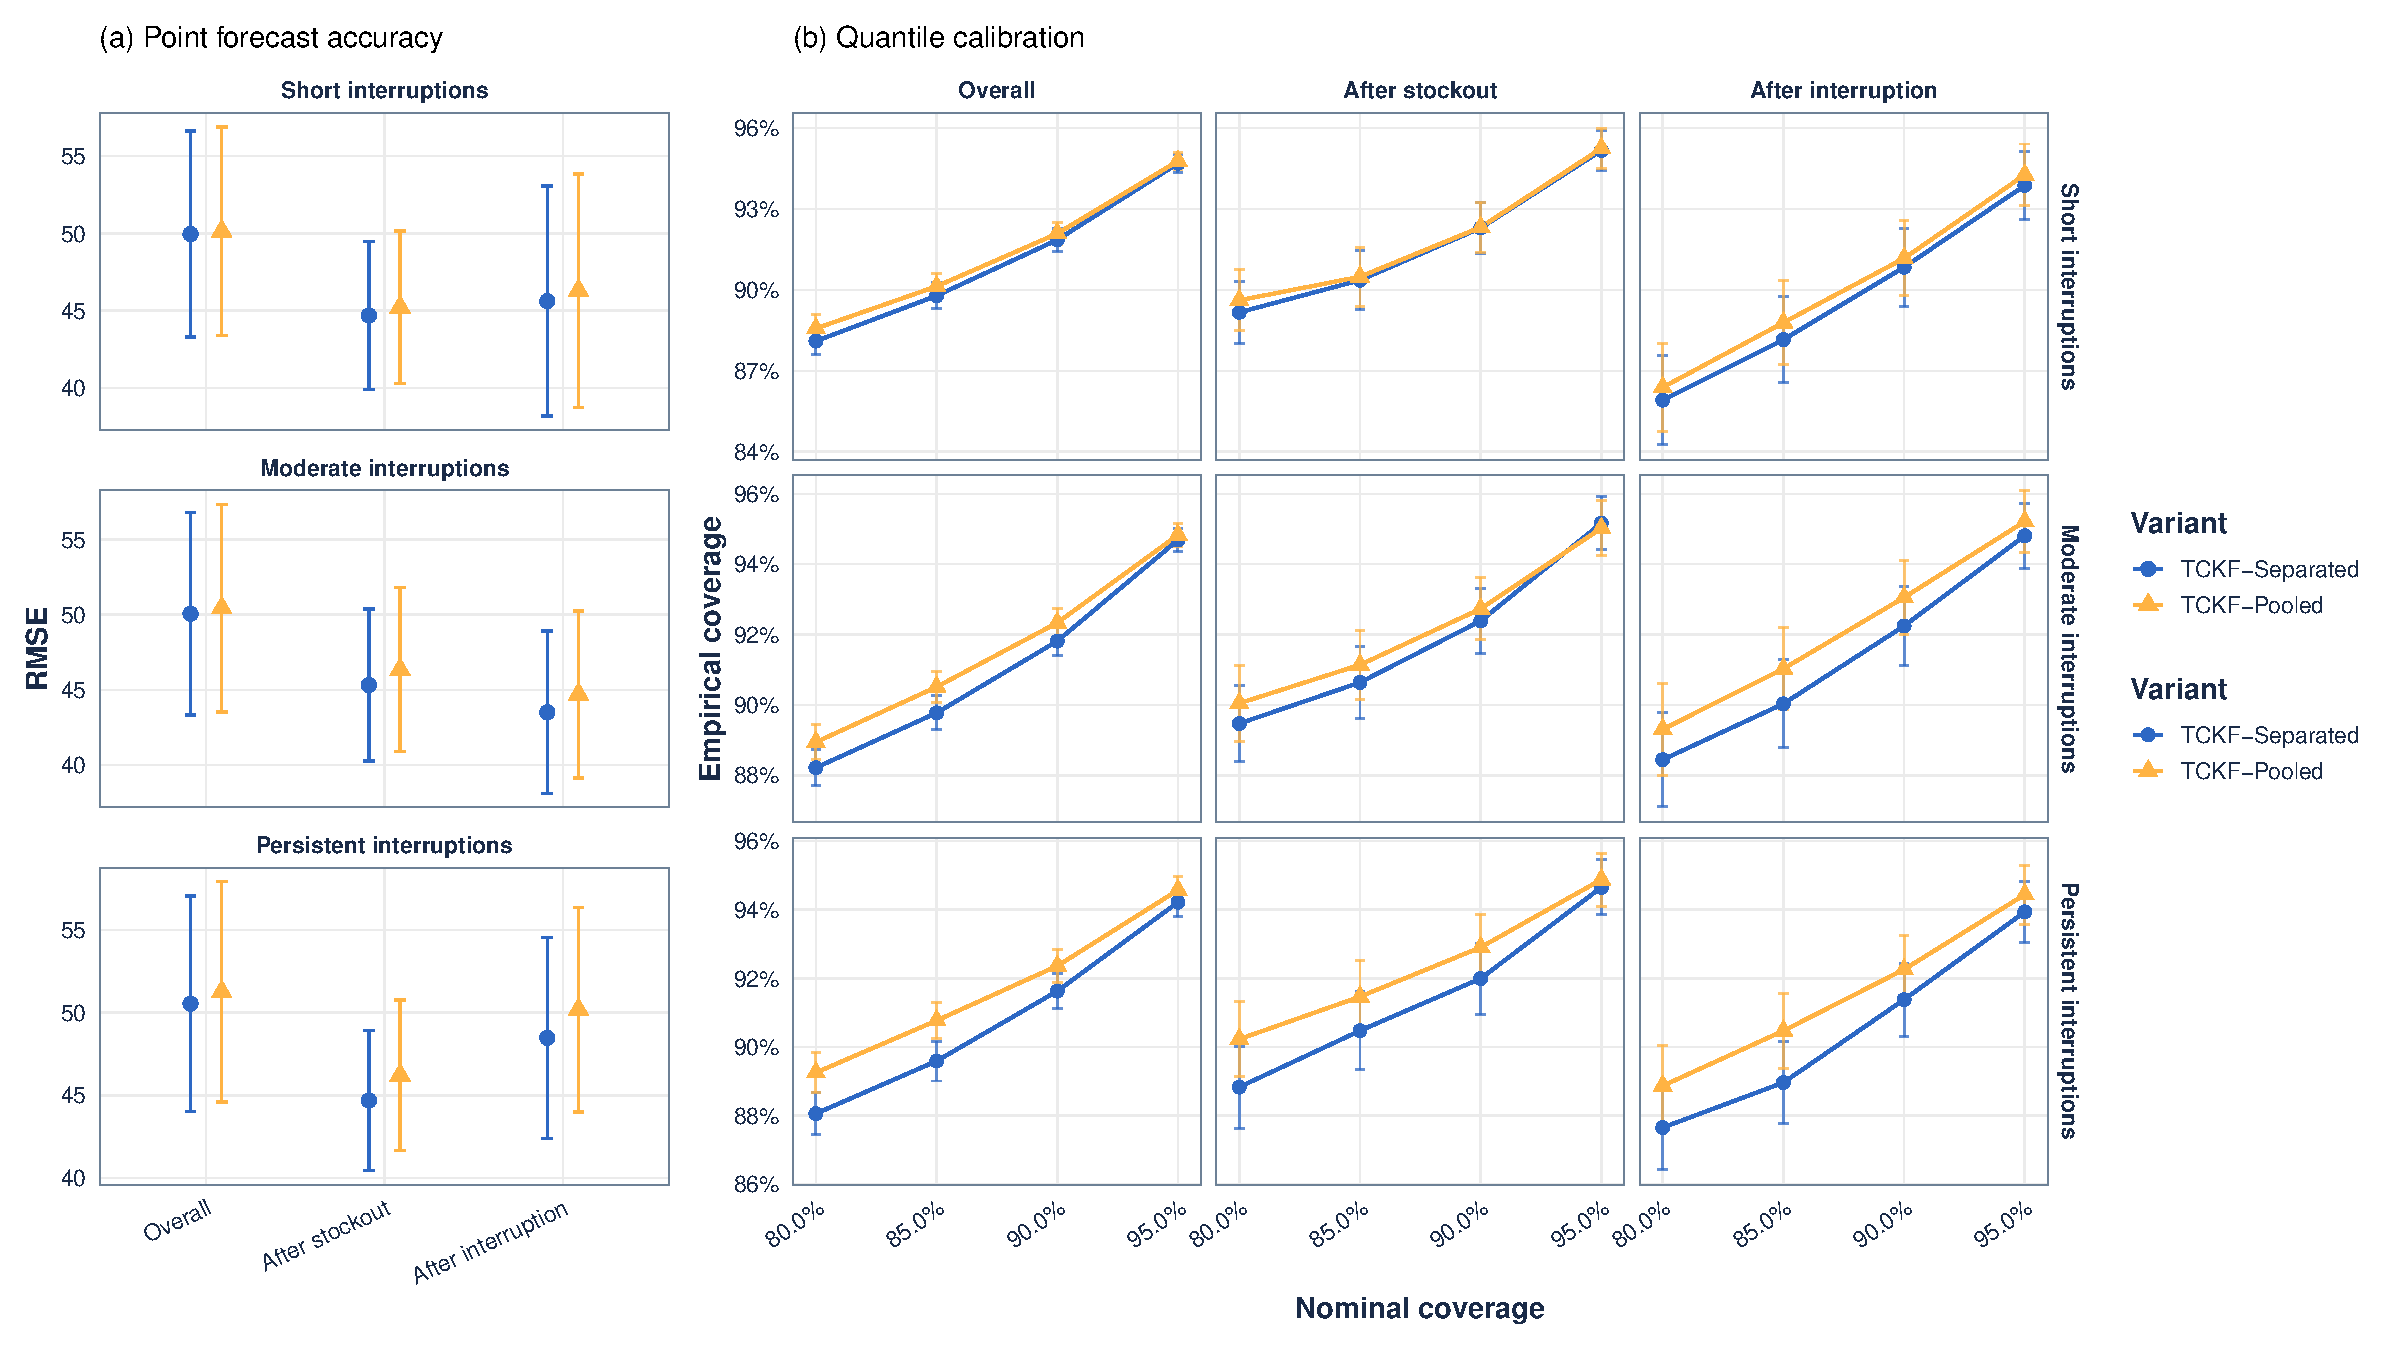
\includegraphics[width=\linewidth,height=0.85\textheight,keepaspectratio]{Main-Paper-Figure-02.pdf}

}

\caption{\label{fig-model_diag_regime_wp2}Point forecast accuracy and
empirical coverage of the regime-separated and pooled TCKF variants
under short, moderate, and persistent service interruptions. Error bars
represent 95\% confidence intervals.}

\end{figure}%

Figure~\ref{fig-model_diag_regime_wp2} shows a consistent direction in
point forecast accuracy: separated TCKF has lower mean RMSE than the
pooled version across the three interruption scenarios. The differences
become larger as interruptions become more persistent. However, their
magnitude remains modest. Under persistent interruptions, mean RMSE
decreases from 51.26 to 50.54 overall, from 46.21 to 44.68 following
stockouts, and from 50.18 to 48.48 following service interruptions.
These correspond to reductions of approximately \(1.4\%\), \(3.3\%\) and
\(3.4\%\), respectively, relative to the pooled version.

The coverage results show a similar but less uniform pattern. Separating
the regimes generally reduces overcoverage at the \(80\%-90\%\)
quantiles, with larger differences under persistent interruptions. For
example, following persistent interruptions, empirical coverage at the
\(90\%\) quantile decreases from \(92.26\%\) for the pooled version to
\(91.38\%\) for separated TCKF, bringing it closer to the nominal level
by 0.88 percentage points. At the \(95\%\) quantile, however, the pooled
version is closer to the nominal level in this scenario. Regime
separation therefore does not improve calibration uniformly across all
quantiles.

These results distinguish the direction of the observed differences from
their magnitude and statistical interpretation. The reductions in RMSE
and changes in coverage are modest. The overlapping confidence intervals
shown in the figure are descriptive and do not constitute a formal test
of the differences between the specifications. Statistically significant
improvement in forecast accuracy or calibration from regime separation
has therefore not been established by this comparison. We interpret the
observed differences as descriptive evidence consistent with the
mechanism discussed in Section~\ref{sec-model_seperate}. The broader
numerical and empirical evaluations assess TCKF as a complete framework
and do not isolate the contribution of regime separation.

The sensitivity results support the parsimonious state specification
used in TCKF. Rolling conformal calibration improves empirical coverage
with little change in point accuracy, while estimating the
uncertainty-inflation weight maintains coverage and keeps RMSE stable.
Full results are reported in \textbf{E-companion, Section 10}.

\section{Experiment setup}\label{sec-experiment_wp2}

We adopt a two-stage experimental design. The numerical experiment
evaluates TCKF against known latent demand, while the empirical
experiment uses monthly LMIS data from Côte d'Ivoire to assess
performance under real-world operational constraints. An overview of the
experimental framework is provided in \textbf{E-companion, Section 4}.

\subsection{Forecasting Methods}\label{forecasting-methods}

We benchmark our TCKF model against a suite of standard statistical
(Naïve, Mean, Exponential Smoothing State Space (ETS), ARIMA,
Syntetos--Boylan Approximation (SBA), and Linear Regression (LR)),
machine learning (LightGBM), and foundational (TimeGPT) models. In the
empirical experiment, we also include operational baselines: the
official LMIS System-Generated Forecast and the human Demand
Planner-Adjusted forecast. Full descriptions of these benchmarks, their
implementations, and parameter settings are detailed in
\textbf{E-companion, Section 2}. These benchmarks were selected based on
prior evidence in contraceptive forecasting \citep{hewage2025}.

Our forecasting target is monthly latent demand for each product at each
facility. We assume no censoring during the forecast horizon because
future stockouts and service interruptions are unknown at the time of
forecasting. For most models, we evaluate versions with and without
regressors that identify the historical censoring regime. The candidate
models are summarised in \textbf{E-companion, Section 2}.

\subsection{Forecasting and inventory
setup}\label{forecasting-and-inventory-setup}

The Côte d'Ivoire family planning supply chain includes healthcare
sites, district-level warehouses, national warehouses, national supply
planners, and donor/programme partners. Healthcare sites record stock
movements, consumption, stockouts, and refill needs, and submit monthly
reports and requests. District and national planners review and
coordinate these requests, while national warehouses distribute stock to
district warehouses and facilities. Donor and programme partners support
upstream procurement and commodity availability. The system is therefore
primarily pull-based because the initial replenishment signal comes from
facilities, but it also includes planner review and adjustment before
stock is distributed. A high-level supply chain map is provided in
\textbf{E-companion, Section 3}.

In line with current practice in Côte d'Ivoire, where healthcare
facilities determine refill quantities and submit monthly forecasts and
order requests one month in advance, we set the forecast horizon to
\(h = 1\). This enables a direct comparison with both System-Generated
and Demand Planner-Adjusted forecasts. In our forecasting setup, we use
a time series cross-validation approach with a rolling-origin and an
expanding training window. For the \textbf{numerical experiment}, each
time series uses the first 70 observations for training, and the next 30
observations for evaluation. For the \textbf{empirical experiment}, the
training period spans from January 2016 to December 2018, and the test
period covers the entirety of 2019. At each iteration, the model is
trained on all data up to time \(t\), and used to forecast the next
period. This setup provides a robust view of forecast accuracy across
varying demand conditions \citep{svetunkov2023}.

To ensure consistency across models, we generate prediction intervals
using conformal prediction. This matches the structure of the proposed
TCKF model, which also uses a conformal prediction layer for uncertainty
estimation. For LMIS forecasts and planner adjustments, which are
provided as point estimates, we apply conformal prediction as post hoc
to produce comparable uncertainty intervals.

For the inventory simulation, we model a monthly periodic-review
lost-sales system with a fixed lead time of one month (\(L=1\)),
consistent with the replenishment cycle in Côte d'Ivoire. At the end of
each month \(t\), after demand is realised, a facility places an order
\(q_t\) that becomes available in month \(t+1\). Replenishment decisions
are based on the inventory position \(IP_t\) (on-hand plus pipeline
stock) \citep{bijvank2011}. With \(L=1\), pipeline stock equals the
order placed in the previous month, and hence \(IP_t = I_t + q_{t-1}\).
Under an order-up-to policy with target level \(U_t\), orders follow
\(q_t=\max{0, U_t - IP_t}\), and any demand exceeding available
inventory is treated as lost sales.

We evaluate a structured set of benchmark replenishment policies that
vary only in how the target level \(U_t\) is determined. These include:
(i) an as-is policy reflecting current LMIS practice (three-month buffer
based on a point forecast) \citep{hewage2025}; (ii) an uncertainty-aware
base-stock policy that sets \(U_t\) using forecast quantiles derived via
conformal prediction \citep{babai2025}; (iii) lost-sales heuristics
commonly used in practice (myopic variants) \citep{bijvank2011}; and
(iv) an oracle benchmark that uses the latent demand process to provide
an upper bound on achievable inventory performance under the same
operating constraints \citep{sachs2014}. We do not attempt to solve for
a globally optimal dynamic inventory policy; rather, these benchmarks
are used to assess how forecast quality and uncertainty quantification
translate into replenishment performance in a standardised lost-sales
setting. Full descriptions of the inventory policies are provided in
\textbf{E-companion, Section 4}.

Alongside the model-based forecasts, we also include the
System-Generated and Demand Planner-Adjusted forecasts in the inventory
simulation to enable a full comparative analysis in empirical
evaluation. We do not use actual stock movement records for inventory
simulation, given the influence of external factors such as delivery
delays and upstream stock availability at district warehouses.

The base case simulation assumes a one-month lead time because the Côte
d'Ivoire LMIS follows a monthly review cycle, where facilities submit
forecasts and order requests one month in advance. Therefore, \(L=1\)
represents the planned replenishment cycle. However, in practice,
replenishment can take longer because of delivery delays, incomplete
fulfilment, or upstream stock availability constraints.

To check the one-month lead-time assumption, we used the stock movement
data to construct an approximate lead-time proxy. We compare the base
case with fixed lead times of two and three months and a stochastic
scenario based on the observed receipt delays. Full details are provided
in \textbf{E-companion, Section 4}.

\subsection{Performance evaluation}\label{performance-evaluation}

We assess point forecast accuracy using Forecast Value Added (FVA) based
on relative RMSE, and probabilistic forecast accuracy using pinball-loss
Skill Scores. Both measures are expressed relative to TCKF, with
positive values indicating better performance. In the numerical
experiment, true demand is known, allowing evaluation in both censored
and uncensored periods. The empirical forecast and inventory comparisons
use uncensored observations, where recorded stock distributed is treated
as observed demand.

For the inventory evaluation, we focus on the trade-off between product
availability, unmet demand and inventory burden. Achieved cycle service
level (CSL) measures the proportion of periods in which opening stock
covers demand, and the lost-demand rate measures the share of demand
left unmet. We report average opening inventory in the numerical
experiment and opening months of stock and proxy opening inventory value
in the empirical experiment. We also translate differences in stockout
exposure into illustrative relative modern contraceptive prevalence rate
(mCPR) loss, benchmarked against TCKF within each policy. The formulas
and proxy-price sources are provided in \textbf{E-companion, Section 5}.

\section{Results}\label{sec-results_wp2}

\subsection{Numerical experiment
setup}\label{numerical-experiment-setup}

The numerical dataset contains 1,000 monthly time series, representing
100 stores and 10 products, each with 100 observations. The series
include intermittent demand, weak and varying seasonal patterns,
stockouts and service interruptions. The data-generating process uses
heavy-tailed innovations, whereas TCKF assumes Gaussian innovations. The
simulated censoring regimes are identified without error. Details of the
data-generation process and the series profiles are provided in
\textbf{E-companion, Section 6}. The effect of regime separation is
isolated through the pooled comparison in Section~\ref{sec-model_diag}.

\subsection{Empirical experiment setup using real-world
data}\label{empirical-experiment-setup-using-real-world-data}

For the empirical evaluation, we used monthly LMIS data from Côte
d'Ivoire covering January 2016 to December 2019. The dataset includes
507 time series across nine contraceptive products, including condoms,
emergency contraceptives, oral pills, injectables, implants, and IUDs.
The target variable is stock distributed, which we treat as observed
demand.

To identify censored demand, we used the stockout-days field and comment
logs written by demand planners. These comments include information on
stockouts, facility closures, delivery delays, untrained staff, upstream
stock availability problems, and other service disruptions. Based on
these fields, we constructed two indicators: one for stockouts and one
for service interruptions. For new product introductions, we imputed
zeros before the first recorded appearance using metadata and site-level
comments.

The real-world series show irregular, intermittent and often weakly
seasonal patterns, consistent with the types of demand considered in the
numerical experiment. The empirical series profiles are provided in
\textbf{E-companion, Section 6}.

\subsection{Forecast performance
evaluation}\label{forecast-performance-evaluation}

In the numerical experiment, we compare the relative forecast
performance of all candidate models against the TCKF benchmark.
Table~\ref{tbl-num_fc_acc_wp2} reports the mean FVA for point forecasts
and the mean Skill Score for different quantile levels. Across both
point and probabilistic forecasts, none of the benchmark models achieves
a positive mean FVA or mean Skill Score. This indicates that, on
average, no method adds value relative to TCKF in the synthetic setting.

\begin{table}[H]

\caption{\label{tbl-num_fc_acc_wp2}Overall forecast performance,
expressed as mean FVA and mean Skill Scores, in the numerical
experiment. Best values in each column are highlighted in bold.}

\centering{

\centering\begingroup\fontsize{6}{8}\selectfont

\resizebox{\ifdim\width>\linewidth\linewidth\else\width\fi}{!}{
\begin{tabular}{>{\raggedright\arraybackslash}p{16em}>{\raggedright\arraybackslash}p{6em}>{\raggedleft\arraybackslash}p{6em}>{\raggedleft\arraybackslash}p{6em}>{\raggedleft\arraybackslash}p{6em}>{\raggedleft\arraybackslash}p{6em}>{\raggedright\arraybackslash}p{6em}}
\toprule
Method & Mean FVA & Mean Skill Score (q80) & Mean Skill Score (q85) & Mean Skill Score (q90) & Mean Skill Score (q95) & Mean Skill Score (q97.5)\\
\midrule
TCKF & \textbf{0.000} & \textbf{0.000} & \textbf{0.000} & \textbf{0.000} & \textbf{0.000} & \textbf{0.000}\\
Censored Linear Regression & -0.271 & -2.979 & -2.532 & -4.136 & -4.538 & -11.654\\
Censored ARIMA & -0.305 & -3.396 & -2.817 & -4.065 & -4.661 & -11.900\\
Censored Mean & -0.465 & -2.698 & -2.217 & -2.628 & -2.993 & -5.279\\
Linear Regression & -0.659 & -3.465 & -2.764 & -4.502 & -4.899 & -12.730\\
\addlinespace
ETS & -0.663 & -4.680 & -3.280 & -4.523 & -4.864 & -10.514\\
Syntetos-Boylan Approx & -0.688 & -4.076 & -3.283 & -4.226 & -4.691 & -8.985\\
ARIMA & -0.759 & -4.425 & -3.627 & -5.357 & -4.922 & -10.278\\
TimeGPT & -0.854 & -4.638 & -3.863 & -6.662 & -10.527 & -34.409\\
LightGBM & -0.916 & -4.245 & -4.004 & -5.380 & -5.528 & -10.587\\
\addlinespace
Mean & -0.945 & -4.906 & -4.194 & -5.118 & -5.073 & -5.750\\
Naive & -1.474 & -6.288 & -4.920 & -5.851 & -6.578 & -11.458\\
Censored TimeGPT & -2.856 & -9.003 & -10.600 & -15.199 & -20.198 & -40.368\\
Censored LightGBM & -4.192 & -25.336 & -29.956 & -45.753 & -74.803 & -158.622\\
\bottomrule
\end{tabular}}
\endgroup{}

}

\end{table}%

In the empirical evaluation, we assess forecast performance using
uncensored observations only, so that accuracy reflects periods where
demand is observed without distortion from stockouts or interruptions.
Table~\ref{tbl-fc_acc_wp2} shows the same overall pattern: no method
improves on TCKF in either FVA or Skill Scores. However, model behaviour
changes in the real setting. Linear Regression, which is comparatively
competitive in the synthetic experiment, performs substantially worse
empirically. This is consistent with the empirical data characteristics.
Most series exhibit moderate-to-low seasonality, and many are
intermittent with low overall demand. These features reduce the
advantage of models that rely on strong trend or seasonal structure and
favour approaches that remain stable under sparse and irregular demand.

The LMIS System-Generated forecast performs similarly to simple
mean-based baselines, which is acceptable as a reference point, but it
remains far from TCKF. Demand planner adjustments consistently reduce
forecast accuracy relative to the system forecast. From a pure
forecasting standpoint, these adjustments do not add value. However, it
remains important to see how these adjustments affect inventory
outcomes, since they may still serve operational purposes beyond
forecast error minimisation.

\begin{table}

\caption{\label{tbl-fc_acc_wp2}Overall forecast performance, expressed
as mean FVA and mean Skill Scores, in the empirical evaluation. Best
values in each column are highlighted in bold.}

\centering{

\centering\begingroup\fontsize{6}{8}\selectfont

\resizebox{\ifdim\width>\linewidth\linewidth\else\width\fi}{!}{
\begin{tabular}{>{\raggedright\arraybackslash}p{16em}>{\raggedright\arraybackslash}p{6em}>{\raggedleft\arraybackslash}p{6em}>{\raggedleft\arraybackslash}p{6em}>{\raggedleft\arraybackslash}p{6em}>{\raggedleft\arraybackslash}p{6em}>{\raggedright\arraybackslash}p{6em}}
\toprule
Method & Mean FVA & Mean Skill Score (q80) & Mean Skill Score (q85) & Mean Skill Score (q90) & Mean Skill Score (q95) & Mean Skill Score (q97.5)\\
\midrule
TCKF & \textbf{0.000} & \textbf{0.000} & \textbf{0.000} & \textbf{0.000} & \textbf{0.000} & \textbf{0.000}\\
ETS & -0.884 & -4.219 & -4.215 & -4.286 & -3.548 & -4.272\\
Mean & -0.885 & -3.688 & -3.799 & -3.738 & -3.760 & -4.415\\
Censored Mean & -0.888 & -3.820 & -3.918 & -3.902 & -4.103 & -4.850\\
Syntetos-Boylan Approx & -0.973 & -4.389 & -4.769 & -4.434 & -4.401 & -4.872\\
\addlinespace
TimeGPT & -1.101 & -5.555 & -6.770 & -8.818 & -14.319 & -21.237\\
Censored LightGBM & -1.172 & -4.169 & -4.347 & -4.348 & -4.280 & -4.957\\
Censored TimeGPT & -1.174 & -5.333 & -6.445 & -8.406 & -13.833 & -20.381\\
ARIMA & -1.176 & -4.674 & -4.930 & -5.141 & -4.649 & -5.396\\
LightGBM & -1.176 & -4.072 & -4.202 & -4.114 & -4.053 & -4.676\\
\addlinespace
Censored ARIMA & -1.189 & -5.207 & -5.580 & -5.781 & -5.197 & -5.684\\
Naive & -1.706 & -4.717 & -4.761 & -4.853 & -4.788 & -5.747\\
Linear Regression & -1.954 & -5.696 & -6.283 & -6.731 & -7.053 & -7.600\\
Censored Linear Regression & -2.006 & -5.994 & -6.636 & -7.221 & -8.046 & -8.280\\
\bottomrule
\end{tabular}}
\endgroup{}

}

\end{table}%

To test whether differences in forecast performance are statistically
significant, we apply the Nemenyi post-hoc test at the 5\% level using
inverted FVA values (i.e., \((1-\text{FVA})\), which is equivalent to a
relative RMSE scale). This transformation is needed because the Nemenyi
procedure ranks methods from smallest to largest values, whereas higher
FVA indicates better performance. By inverting FVA, better models have
smaller values and therefore better (lower) ranks, making the ranking
direction consistent with the test.

Figure~\ref{fig-fva_nemenyi_wp2} presents the results as a
critical-difference style rank plot for the numerical (left) and
empirical (right) experiments. Each method is shown with its average
rank, and the horizontal bar indicates the 95\% confidence interval for
that rank. The shaded grey band marks the 95\% confidence interval of
the best-ranked method. Any method whose confidence interval overlaps
this grey band is not significantly different from the top performer;
methods whose intervals lie fully outside the band are significantly
worse. Across both settings, TCKF achieves the best (lowest) average
rank and its grey-band interval does not overlap with any other method,
indicating that TCKF is significantly better than all alternatives at
the 5\% level. In the numerical experiment, SBA ranks relatively well
compared to many benchmarks, which is notable given its design for
intermittent demand and consistent with the high intermittency embedded
in the synthetic data. In several model families (e.g., Mean and ARIMA),
adding censoring information improves performance relative to their
uncensored variants, suggesting that explicitly encoding censored-period
structure can reduce bias in demand estimation. The same pattern is
weaker for LightGBM, where the censored version offers only marginal
improvement.

\begin{figure}

\centering{

\pandocbounded{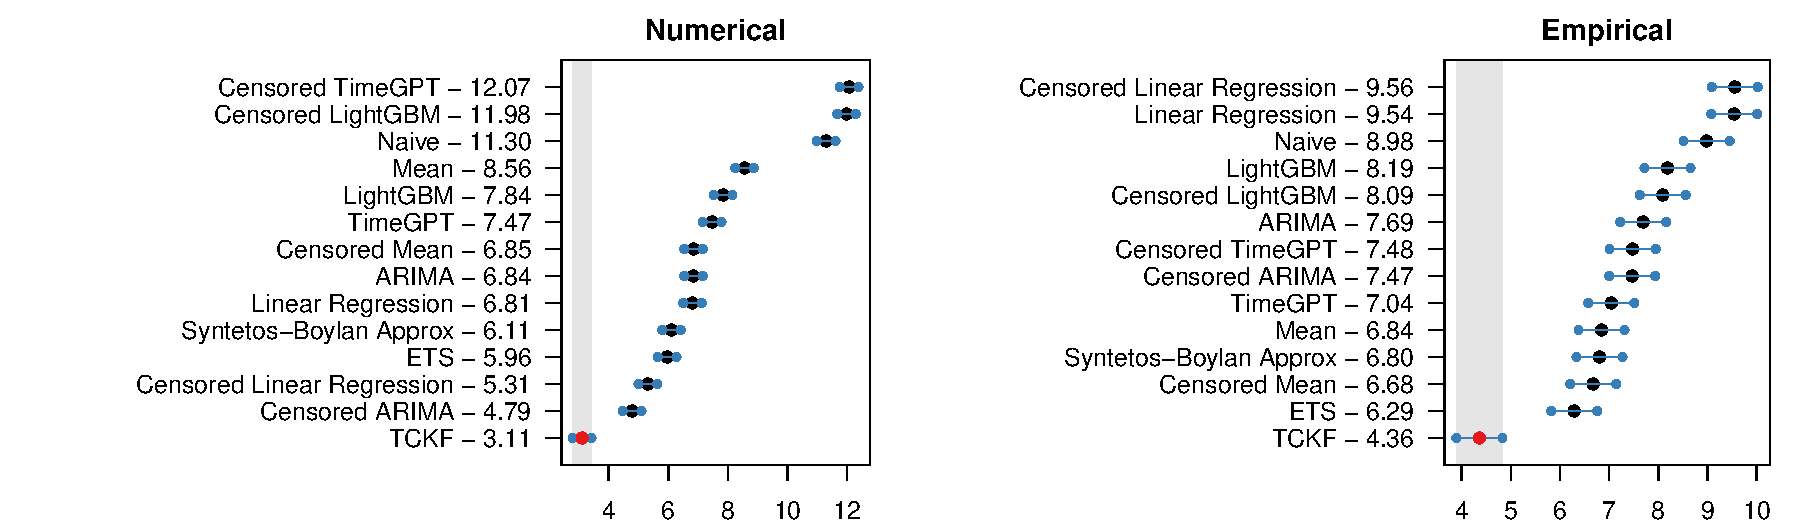
\includegraphics[keepaspectratio]{Main-Paper-Figure-03.pdf}}

}

\caption{\label{fig-fva_nemenyi_wp2}Nemenyi post-hoc test with 95\%
confidence level on inverted FVA values.}

\end{figure}%

\subsection{Inventory performance}\label{inventory-performance}

We first evaluate inventory performance in the numerical experiment,
where true demand is known. This allows us to assess whether each
forecasting method can support service improvements without requiring
excessive inventory. Since the objective of the numerical experiment is
to compare forecast-policy behaviour under controlled conditions, we
interpret the results as service--inventory trade-offs rather than as
direct operational stock targets.

Figure~\ref{fig-num-csl-avg-inventory} shows the trade-off between
achieved CSL and average opening inventory across replenishment
policies. Points closer to the upper-left indicate better performance,
as they provide higher service with lower inventory. The as-is policy
generally produces higher CSL, but it also requires higher inventory
because it follows a multiplier-based stock target. This is expected, as
the three-month target used in practice is designed to cover the review
period, the expected lead time, and a safety buffer.

For the myopic and quantile-based policies, average inventory can be
lower than the three-month target. This should not be interpreted as
contradicting the country policy. These policies do not impose the
three-month multiplier as a fixed rule. Instead, they test whether
forecast-driven replenishment can achieve acceptable service with a
lower stock burden under controlled supply conditions. Therefore, lower
inventory levels under these policies should be interpreted as simulated
efficiency gains, not as direct recommendations to reduce operational
buffers without considering lead-time uncertainty.

\begin{figure}[htbp]

\centering{

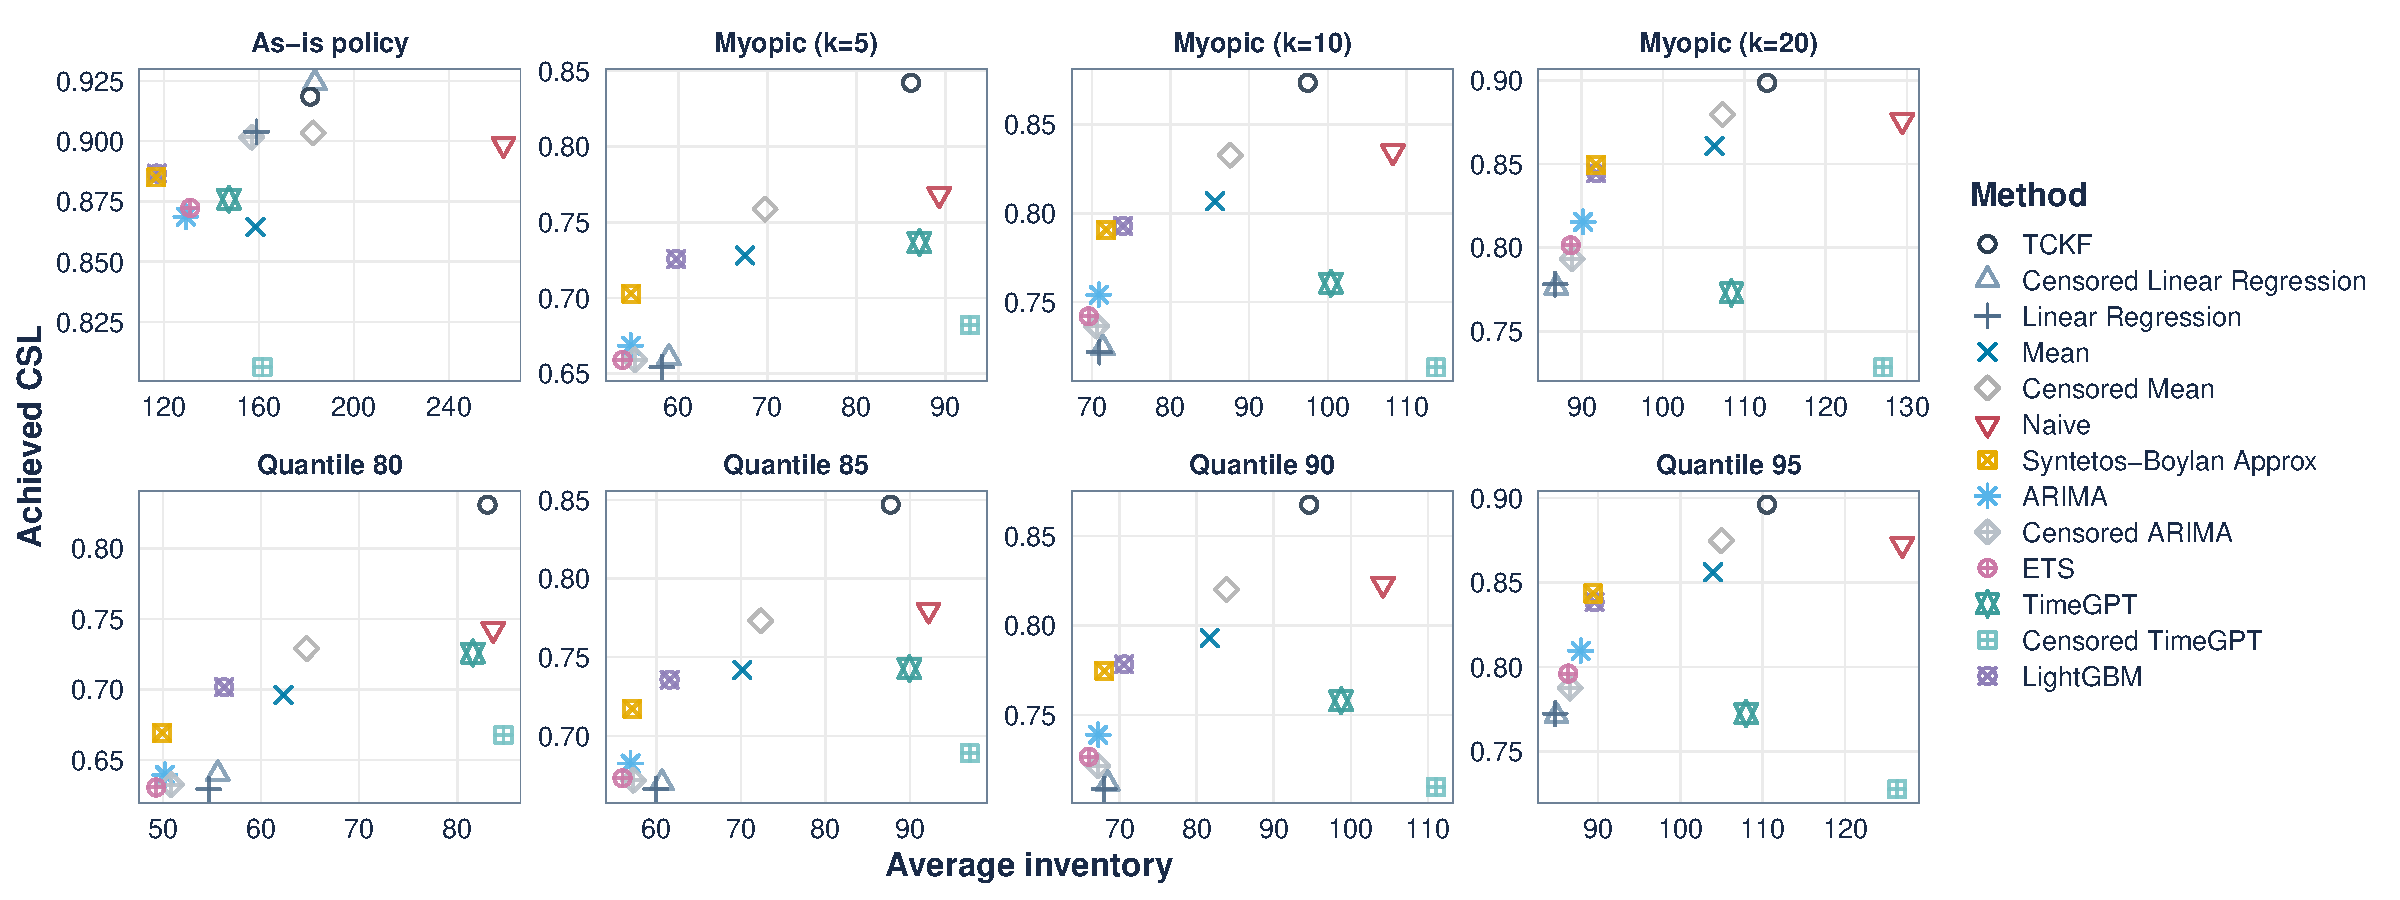
\includegraphics[width=\linewidth,height=0.75\textheight,keepaspectratio]{Main-Paper-Figure-04.pdf}

}

\caption{\label{fig-num-csl-avg-inventory}Numerical inventory trade-off
between achieved cycle service level (CSL) and average inventory across
replenishment policies.}

\end{figure}%

The results show that TCKF is consistently close to the efficient
frontier. Under the as-is policy, Censored Linear Regression achieves a
slightly higher CSL than TCKF, but with a similar or slightly higher
inventory level. Across the myopic and quantile-based policies, TCKF
generally achieves higher service than most benchmark methods for a
comparable inventory burden. In particular, under the quantile policies,
TCKF maintains higher CSL while avoiding the excessive inventory levels
observed for some benchmarks such as Naive and Censored TimeGPT. This
suggests that the main value of TCKF is not simply higher stockholding,
but a more efficient translation of forecast uncertainty into
replenishment decisions. The detailed numerical results, including
lost-demand rates and average inventory values for all forecast-policy
combinations, are reported in \textbf{E-companion, Section 7}.

We next evaluate how the empirical forecasts translate into inventory
outcomes. In the empirical setting, the products are real contraceptive
commodities, so we can extend the numerical analysis by attaching
product-level proxy unit prices to opening stock. These prices are used
only as proxy values, not as audited procurement costs. This allows us
to compare whether service improvements are achieved with proportionate
inventory investment or through substantial stock accumulation. We
therefore report achieved CSL and lost-demand rate against total proxy
opening inventory value, and then translate stockout differences into
relative mCPR loss. The detailed policy-level results are reported in
\textbf{E-companion, Section 7}.

Figure~\ref{fig-emp-csl-proxy-inventory-value} reports achieved CSL
against total proxy opening inventory value. The as-is policy gives an
important benchmark because it is closest to the current three-month
stock logic. Under this policy, the System-Generated forecast achieves a
higher CSL than TCKF, 0.937 compared with 0.918. This result is not
unexpected because both the as-is policy and the System-Generated
forecast are close to moving-average, rule-based planning logic. In
other words, the System-Generated forecast is well matched to the as-is
multiplier rule and should be treated as a strong operational baseline
in this specific setting.

However, CSL should not be interpreted without the corresponding
inventory burden. Demand Planner forecasts usually achieve the highest
CSL, but with much higher stockholding. Under the as-is policy, Demand
Planner reaches a CSL of 0.987, but the total proxy opening inventory
value increases to about USD 607k, compared with USD 449k for the
System-Generated forecast and USD 404k for TCKF. In opening months of
stock, this corresponds to 5.43 months for Demand Planner, 3.43 for
System-Generated, and 3.40 for TCKF. Therefore, the higher service level
from planner adjustment is partly achieved through substantially higher
stockholding. In a resource-constrained supply chain, this matters
because stock held at one facility can reduce availability elsewhere.

\begin{figure}[htbp]

\centering{

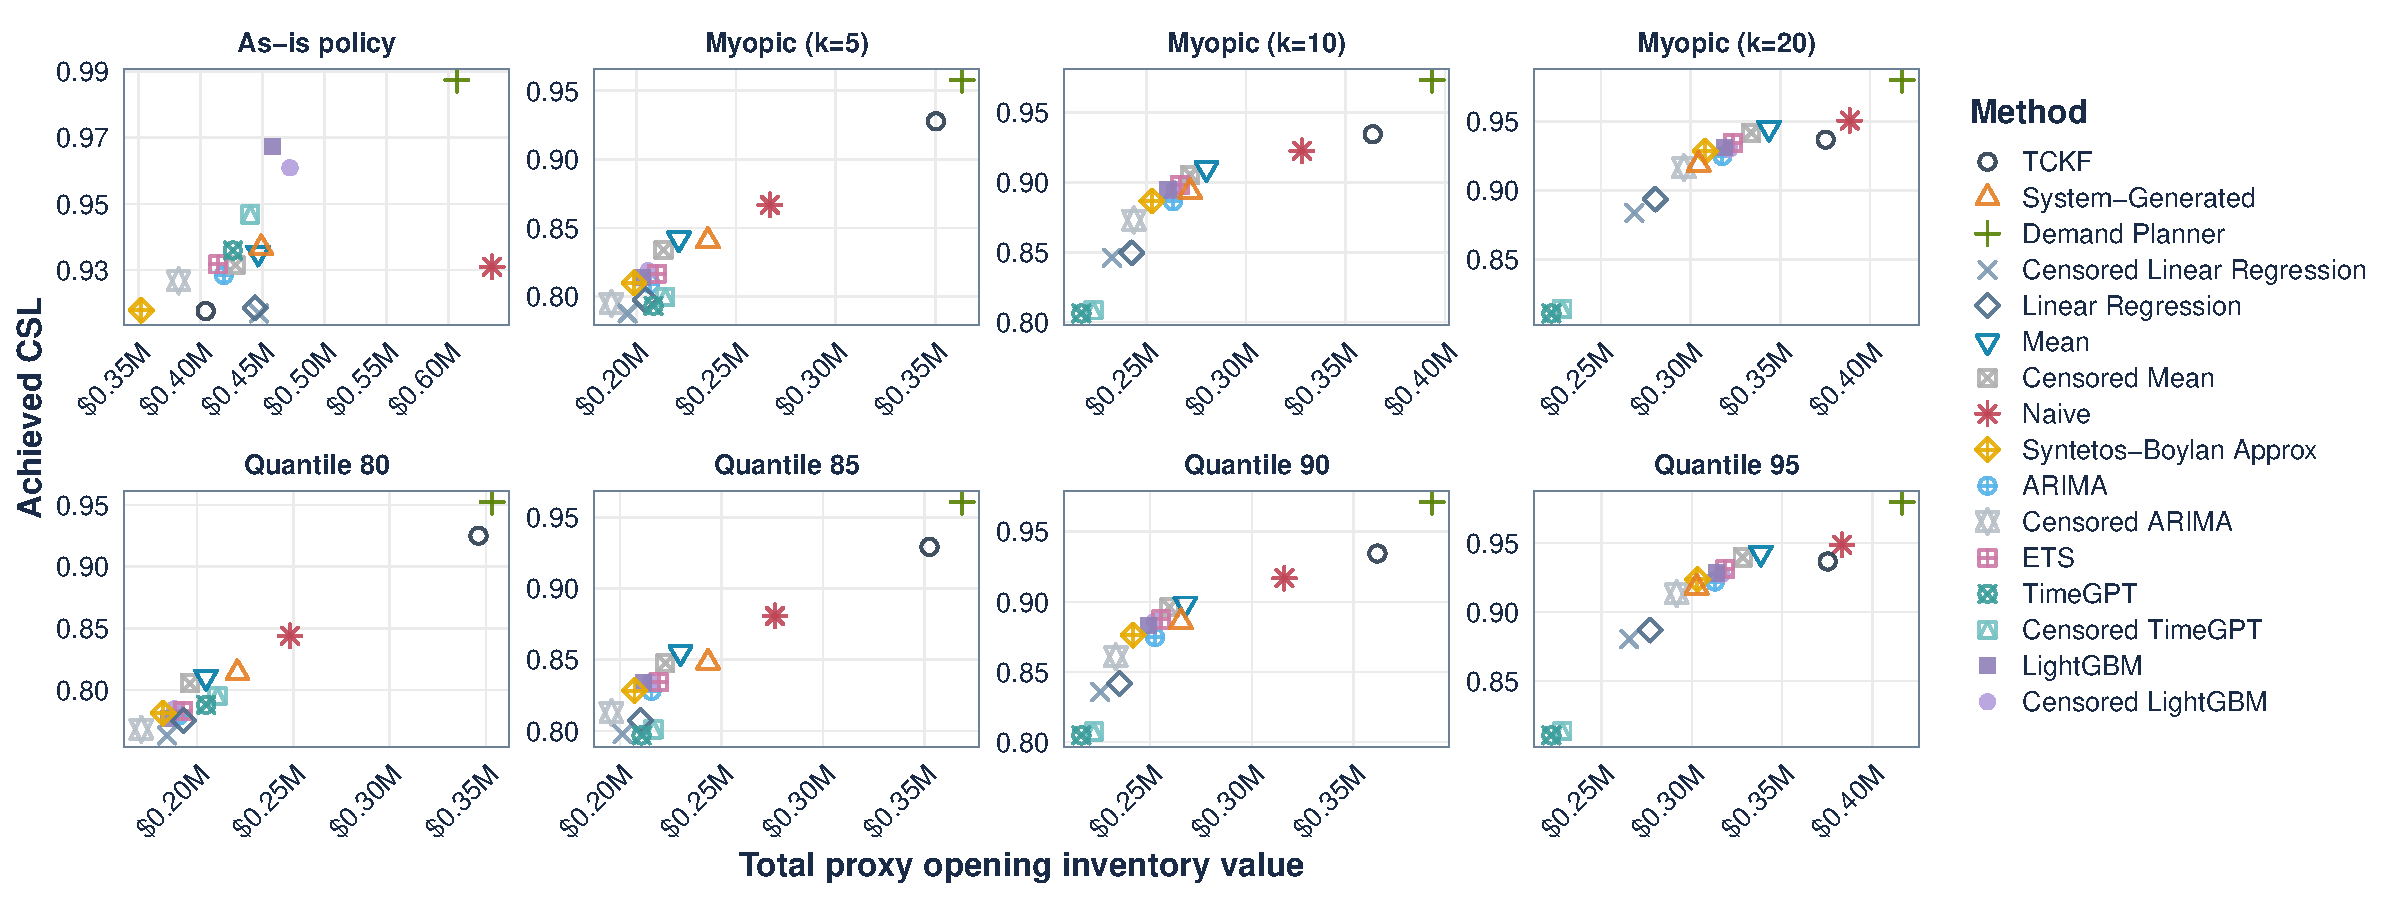
\includegraphics[width=\linewidth,height=0.75\textheight,keepaspectratio]{Main-Paper-Figure-05.pdf}

}

\caption{\label{fig-emp-csl-proxy-inventory-value}Empirical inventory
trade-off between achieved cycle service level (CSL) and total proxy
opening inventory value across replenishment policies.}

\end{figure}%

For sparse and intermittent products, the fixed multiplier in the as-is
policy can produce low stock targets when the point forecast is small,
leaving limited protection against occasional demand spikes. The Copper
T IUD and Implanon examples and the complementary lost-demand results
are reported in \textbf{E-companion, Section 8}.

Finally, Figure~\ref{fig-emp-mcpr-loss-opening-mos} translates stockout
differences into relative mCPR loss and compares them with opening
months of stock. We report this only for the empirical experiment
because this translation is meaningful only in the real product setting,
where stockouts correspond to interruptions in contraceptive access. In
this analysis, relative mCPR loss should therefore be interpreted as a
public-health translation of access disruption, not as a direct measure
of physical lost units.

The mCPR results reinforce the same trade-off. Because relative mCPR
loss is benchmarked against TCKF within each policy, TCKF is normalised
to zero. Under the as-is policy, both operational baselines show lower
relative mCPR loss than TCKF: approximately -0.011 for System-Generated
and -0.041 for Demand Planner. This reflects their lower stockout rates
under the as-is rule. However, this advantage is not free. Demand
Planner achieves the largest reduction in relative mCPR loss while
holding substantially more stock.

Under the quantile policies, the interpretation changes. For example,
under the 90th percentile policy, System-Generated has a positive
relative mCPR loss of about 0.028 compared with TCKF, while Demand
Planner has a negative relative mCPR loss of about -0.021. Under the
95th percentile policy, System-Generated remains worse than TCKF in
relative mCPR terms, about 0.011, while Demand Planner remains better,
about -0.025, but again with a higher inventory burden.

\begin{figure}[htbp]

\centering{

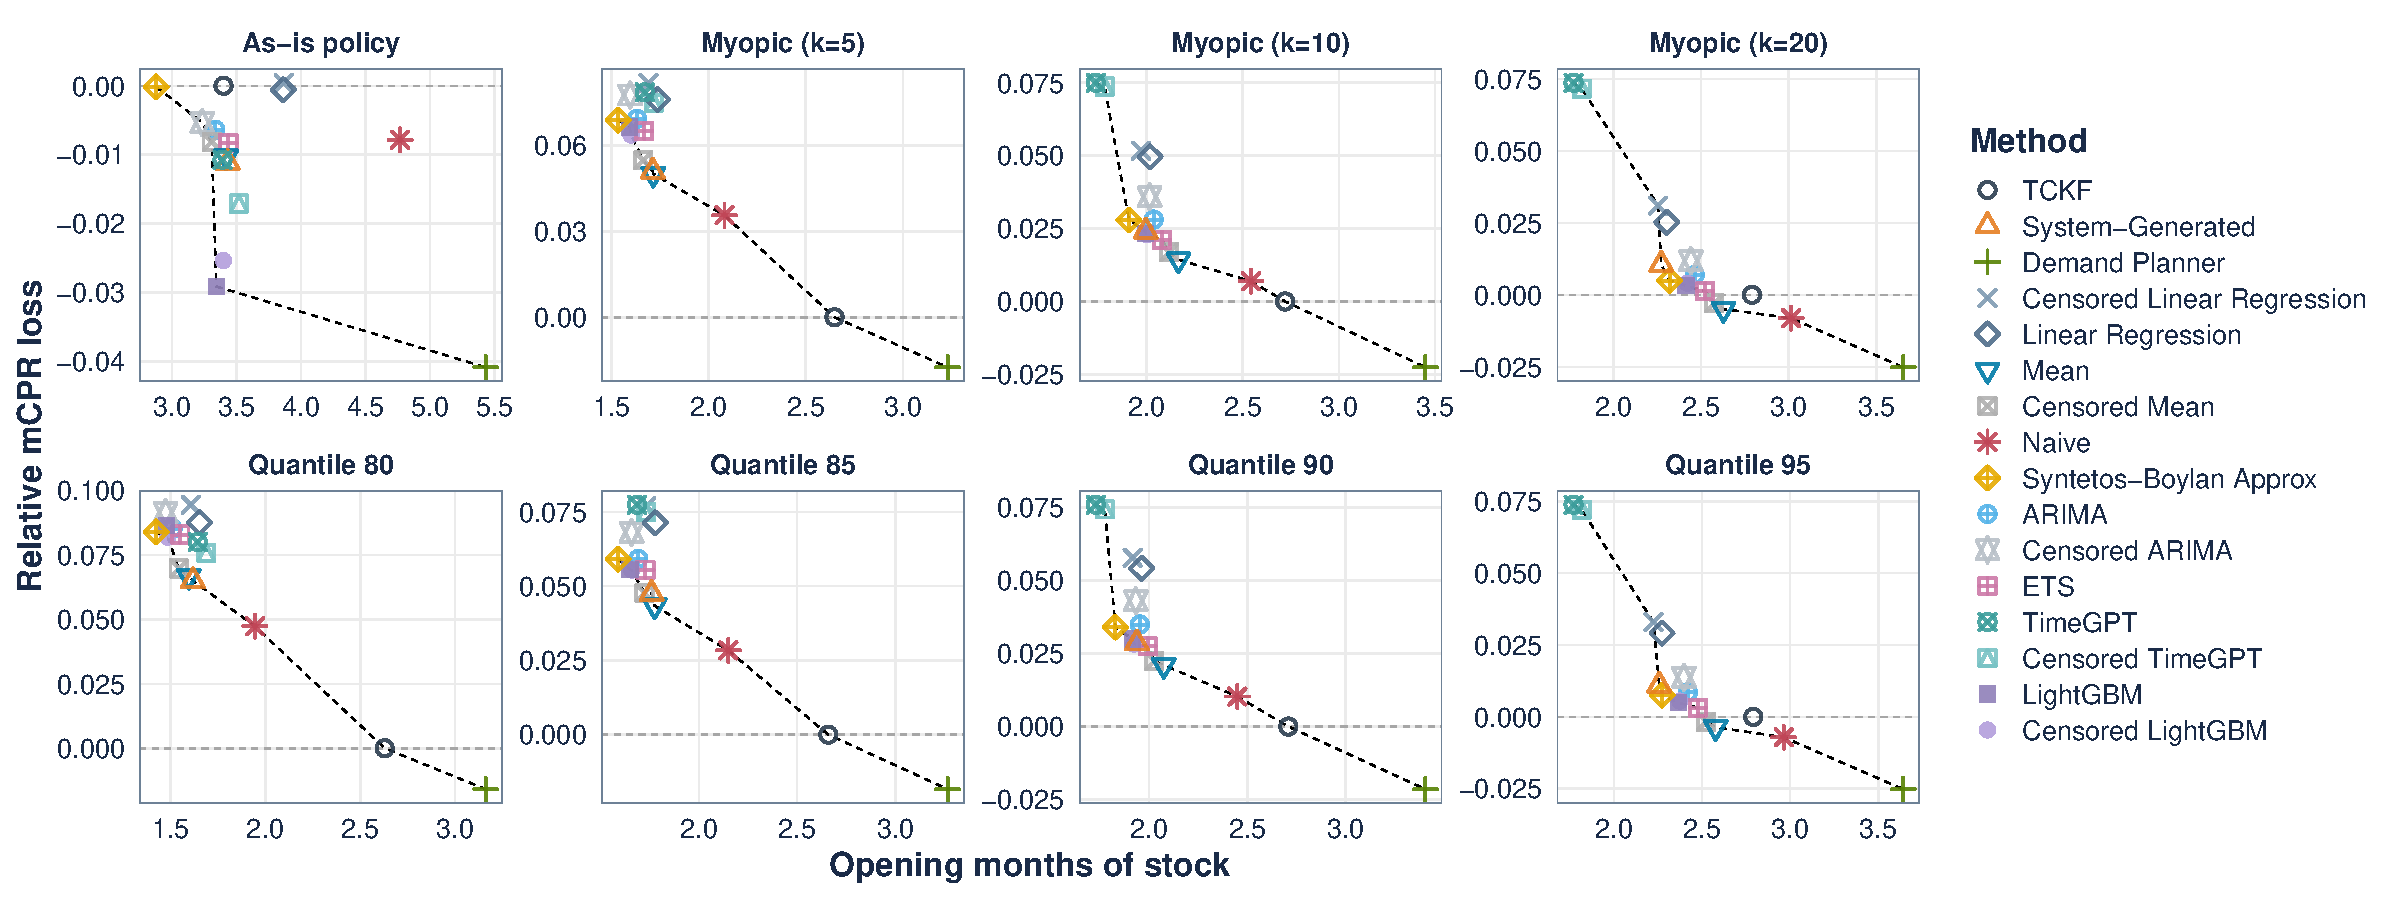
\includegraphics[width=\linewidth,height=0.75\textheight,keepaspectratio]{Main-Paper-Figure-06.pdf}

}

\caption{\label{fig-emp-mcpr-loss-opening-mos}Empirical public-health
trade-off between relative mCPR loss and opening months of stock across
replenishment policies.}

\end{figure}%

\subsection{Lead-time sensitivity
analysis}\label{lead-time-sensitivity-analysis}

To assess the robustness of the reported service levels to the fixed
lead-time assumption, we reran the empirical inventory simulation under
longer and stochastic replenishment delays. In this analysis, we keep
the forecasting inputs and replenishment policies unchanged and vary
only the receipt delay. This allows us to isolate how lead-time
uncertainty affects achieved CSL.

Figure~\ref{fig-leadtime_csl_sensitivity} shows that the fixed one-month
lead time is an optimistic base-case assumption. Across almost all
policies, achieved CSL declines when the lead time is increased from one
to two months, and declines further under a three-month lead time. This
confirms that replenishment timing is an important driver of service
performance and that the absolute CSL values in the base-case simulation
should be interpreted as controlled, forecast-driven outcomes rather
than direct estimates of realised operational service levels.

\begin{figure}[htbp]

\centering{

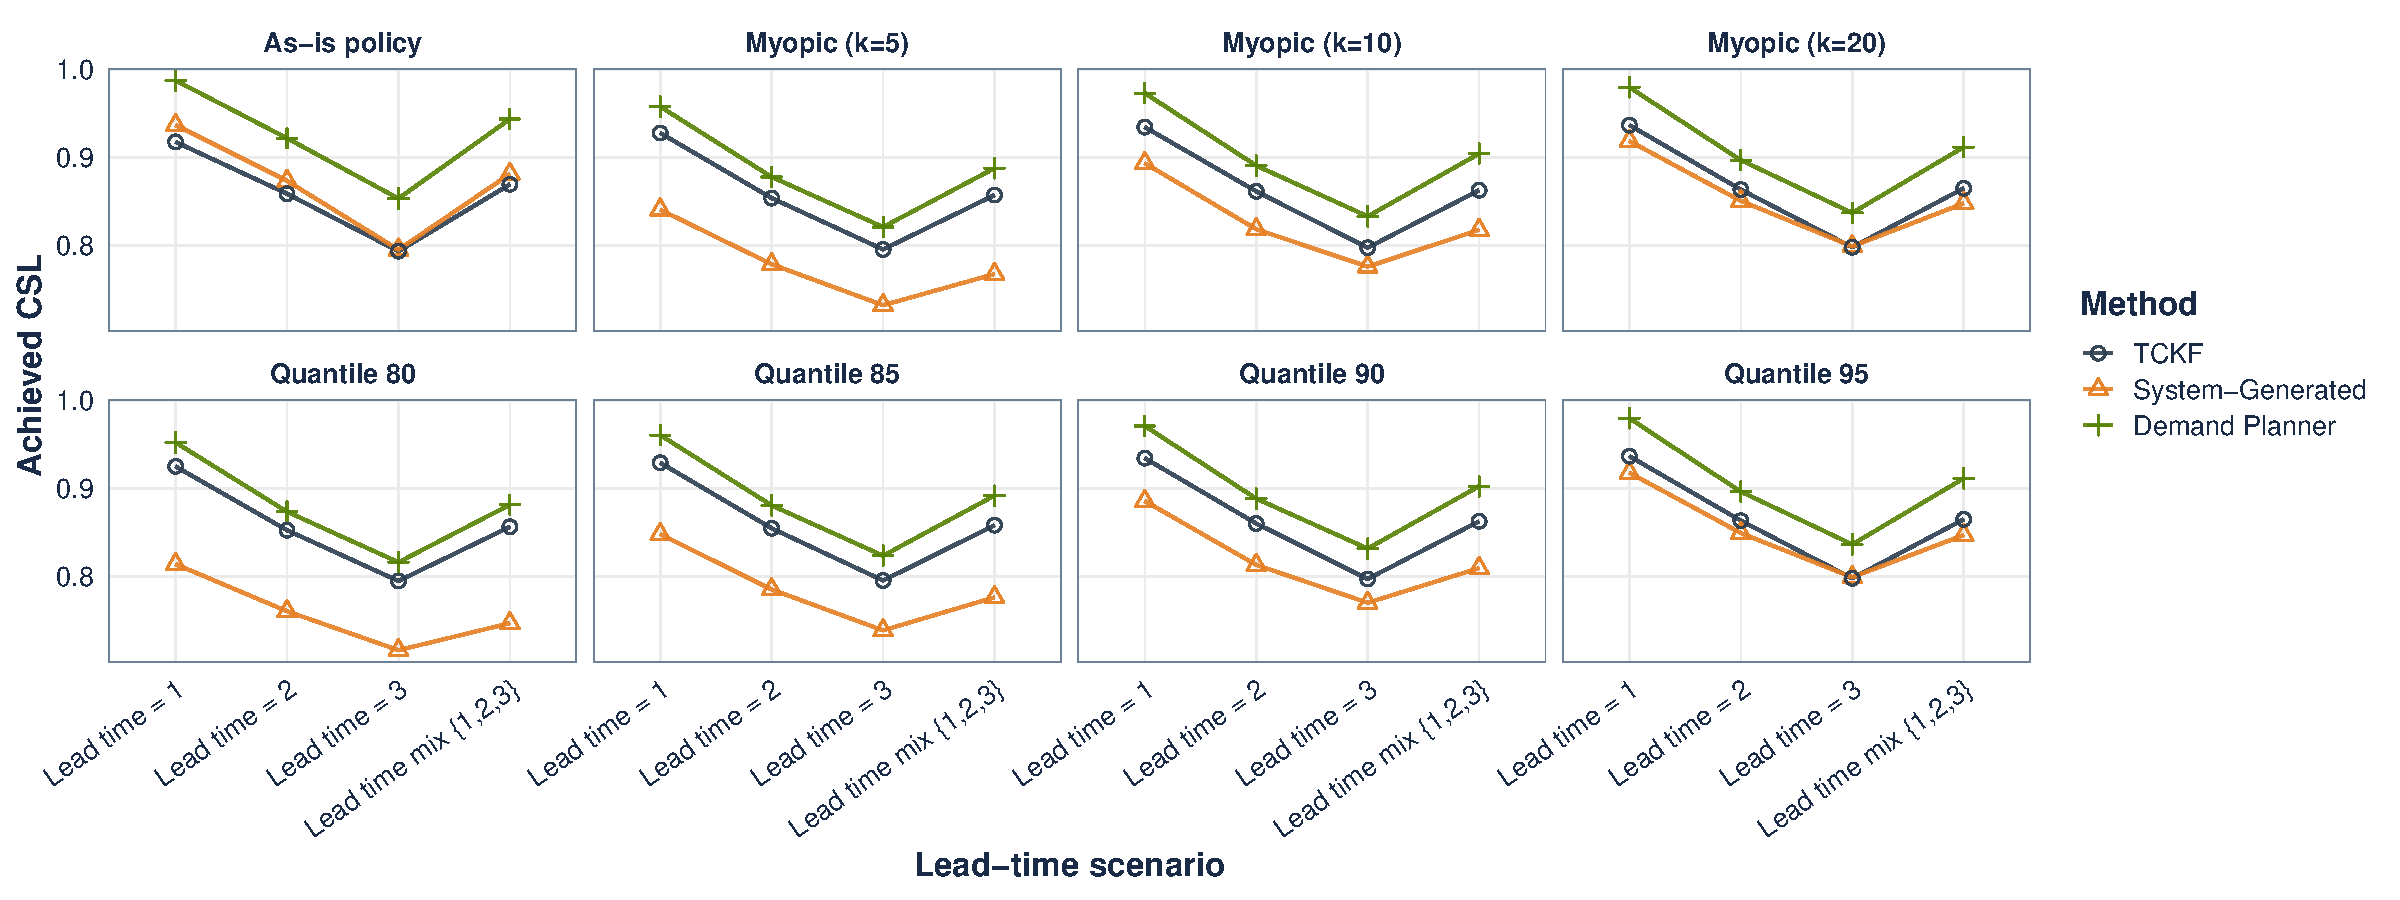
\includegraphics[width=\linewidth,height=0.75\textheight,keepaspectratio]{Main-Paper-Figure-07.pdf}

}

\caption{\label{fig-leadtime_csl_sensitivity}Sensitivity of achieved
cycle service level (CSL) to alternative lead-time assumptions in the
empirical inventory simulation.}

\end{figure}%

We also compare the simulated service levels with the observed achieved
CSL from the original LMIS stock movement data. Here, achieved CSL is
calculated as the proportion of product--facility--month records without
a stockout or service interruption. We use this as an availability-based
benchmark, not as a true demand fill rate, because true demand is
unobserved during stockouts and interruptions. The observed overall
achieved CSL is 0.838, which is lower than most simulated CSL values
under the fixed one-month lead-time setting. This supports the
interpretation that the base-case simulation is optimistic and should be
read as a controlled forecast-policy comparison rather than a direct
estimate of realised service performance. The detailed product-level
summary statistics are reported in \textbf{E-companion, Section 9}.
Notably, the achieved CSL under the stochastic lead-time setting is
closer to this observed empirical CSL, suggesting that allowing lead
times to vary provides a more realistic service-level benchmark than the
fixed one-month base case.

However, the main operational interpretation remains broadly unchanged.
Demand Planner forecasts generally maintain the highest CSL across
lead-time scenarios, but this should be interpreted together with the
much larger inventory burden reported earlier. TCKF remains more robust
than the System-Generated forecast in most policies, particularly under
the quantile-based policies where uncertainty calibration is important.
The stochastic lead-time scenario falls between the fixed one-month and
fixed three-month cases, as expected, because it combines shorter and
longer replenishment delays according to the empirical delay
distribution.

\section{Discussion and conclusion}\label{sec-discussion_wp2}

\subsection{Findings and managerial
implications}\label{findings-and-managerial-implications}

The main methodological contribution of this study is TCKF, a
probabilistic framework for estimating censored demand and supporting
inventory decisions in FPSCs. TCKF extends the classical TKF in two main
ways. First, it distinguishes stockouts from service interruptions and
treats them differently in the state update. Second, it adds conformal
calibration to represent the uncertainty remaining after censored demand
estimation. These extensions address different issues: regime separation
determines how censored observations inform the demand state, while
conformal calibration adjusts the uncertainty estimates used in
replenishment decisions.

The discussion in Section~\ref{sec-model_seperate} explains the
reasoning behind regime separation. During a known service interruption,
the recorded zero provides no additional demand information under the
stated conditions, which motivates skipping the measurement update. The
numerical comparison shows modest reductions in mean RMSE relative to an
otherwise identical pooled specification, with larger differences under
persistent interruptions. Coverage is generally closer to nominal levels
at the \(80\%-90\%\) quantiles, although this pattern does not hold
uniformly. These observations are consistent with the proposed
mechanism, but the diagnostic comparison does not establish
statistically significant improvement from regime separation, as
discussed in Section~\ref{sec-model_diag}.

The conformal layer addresses the remaining forecast uncertainty.
Rolling calibration improves coverage without materially changing point
accuracy, while uncertainty inflation allows intervals to widen when
reliable observations remain unavailable. TCKF therefore extends
existing TKF-based approaches by addressing both the information
contained in different censoring regimes and the calibration of forecast
uncertainty \citep{trapero2024}. The broader numerical experiment
evaluates these features together against known demand. TCKF performs
well on point and probabilistic forecast measures and remains close to
the efficient service-inventory frontier, but these results cannot be
attributed to regime separation alone.

The empirical results show that inventory value depends on how forecasts
are used in replenishment. These empirical inventory comparisons are
interpreted descriptively and do not establish statistically significant
gains attributable to regime separation. Under the as-is policy, the
System-Generated forecast performs competitively. This policy applies a
fixed multiplier to a point forecast and does not use TCKF's uncertainty
estimates. Under quantile-based policies, TCKF's benefit relative to the
System-Generated forecast becomes clearer, particularly in achieved CSL
and relative mCPR loss. Lost-demand rate does not always follow the same
ordering, so both stockout frequency and unmet demand volume should be
considered. Demand Planner forecasts generally achieve the highest
service levels but require substantially more inventory. This pattern is
consistent with upward adjustments intended to protect service against
uncertainty \citep{fahimnia2023}, which can increase inventory burden
where stock and funding are limited \citep{natarajan2014}. Since
complete holding, expiry, shortage and opportunity cost data are
unavailable, we identify service-inventory trade-offs rather than a
cost-optimal policy. Relative mCPR loss translates stockout exposure
into potential contraceptive-access consequences and should not be
interpreted as a causal estimate of health outcomes.

The main managerial implication follows directly: the reason for a
censored observation should be retained in LMIS records and used in
forecasting, since a stockout and an interruption carry different
information about unmet demand. The practical value of separating them
depends on the frequency and duration of interruptions and the
reliability of their identification. The observed gains are modest but
larger under persistent interruptions, suggesting that regime separation
may be more useful where interruptions repeatedly affect the demand
history. Its operational value also depends on whether replenishment
decisions use the resulting forecast information.

Feasibility and scalability depend on the available data and technical
capacity. TCKF remains a parsimonious state-space method that uses
routine LMIS variables and could be incorporated into existing
forecasting and dashboard workflows, including platforms such as DHIS2
\citep{DHIS2_DigitalHealthWeek2024}. Where records already distinguish
the two regimes, implementation may be easier. Otherwise, additional
data recording, validation and staff training may outweigh modest
forecasting gains. Deployment would require technical integration, local
validation and phased implementation. We do not assess these costs or
establish cost-effectiveness, and improved forecasts alone cannot
overcome supply constraints.

\subsection{Limitations and future research
directions}\label{limitations-and-future-research-directions}

The direction of the observed differences motivates further research on
the value of regime separation. Larger gains might arise where
interruptions affect more of the demand history, although this remains
to be tested. Future studies could examine different interruption
patterns and country settings, assess sensitivity to classification
errors, and evaluate whether improvements translate into better
contraceptive availability at an acceptable implementation and inventory
cost. These investigations should also consider the model assumptions
that may influence its performance. First, TCKF assumes Gaussian state
and observation innovations for tractability, whereas demand may exhibit
skewness or heavy tails. Conformal calibration adjusts forecast
intervals but does not remove the distributional assumptions used in the
state updates. Future research could therefore explore alternative
demand distributions and derive the corresponding conditional
expectations for censored observations.

Second, our implementation assumes additive time series components,
following the standard structure of Tobit Kalman Filters. However, in
many real-world healthcare settings, demand patterns may exhibit
multiplicative seasonality, particularly when demand variability grows
with the level. Extending this framework to handle multiplicative
structures would improve its generalisability.

Third, although earlier studies such as \citet{hewage2025} and
\citet{bilal2025} have shown the importance of contextual factors like
healthcare campaigns or awareness programmes, our current model does not
incorporate such covariates. Given the operational importance of these
events, future work could investigate how to integrate such contextual
signals, either as exogenous regressors or through hierarchical
modelling approaches.

While TCKF effectively recovers latent demand lost to stockouts and
service interruptions, it relies on the assumption that the recorded
data itself is fundamentally accurate. In reality, LMIS data is
frequently subject to recording errors, phantom stock, and reporting
lags. Addressing this broader data-quality bias may require additional
data audits and dedicated structural modelling \citep{deboeck2023}.

Our current model assumes that demand censored due to stockouts or
service interruptions is lost permanently, without influencing
subsequent periods. However, in real-world settings, unmet demand may
manifest as a delayed or ``bounce-back'' demand in future periods.
Capturing such lagged effects would require a structural extension of
the state-space model, for instance, incorporating autoregressive lags
of censored demand signals or modeling latent demand recovery processes.
While this is outside the scope of the present work, future research
could investigate these extensions to further improve the reliability
and accuracy in censored-demand forecasting.

Finally, our evaluation focused on assessing the TCKF against current
practice at the healthcare site level, using monthly,
product--facility--level data and a one‐month‐ahead forecast horizon to
reflect operational realities. While this setup aligns closely with
existing decision cycles in Côte d'Ivoire's FPSC, future research could
explore TCKF's performance under alternative temporal granularities
(e.g., weekly, quarterly) and longer forecast horizons using real‐world
data, to assess its robustness across different planning contexts.

\section*{Data availability statement}\label{reproducibility}
\addcontentsline{toc}{section}{Data availability statement}

Code, data, and Quarto source files will be publicly available in the
\href{https://github.com/chamara7h/Estimating-censored-demand-in-family-planning-supply-chains}{GitHub
repository}.

\section*{Acknowledgements}\label{acknowledgements}
\addcontentsline{toc}{section}{Acknowledgements}

This research was supported by a fully funded PhD studentship from the
Welsh Graduate School for the Social Sciences (WGSSS). We thank the
Senior Editor and anonymous reviewers for their constructive feedback.

\section*{References}\label{references}
\addcontentsline{toc}{section}{References}

\renewcommand{\bibsection}{}
\bibliography{references.bib}





\end{document}
